
%Le parole italian ed english istruiscono il tex a sillabare una porzione di testo con le regole rispettivamente in italiano ed inglese. Per passare da italiano ad inglese è sufficiente utilizzare il comando \selectlanguage{english}, per tornare poi all'italiano \selectlanguage{italian}
\documentclass[12pt,a4paper,oneside,english,italian]{book} 

% Usare "oneside" invece di "twoside" nelle bozze, per risparmiare carta: "twoside" produce diverse pagine bianche alla fine dei capitoli.

%Questo pacchetto consente di impostare i margini del documento. La prola headsep sta indicare l'altezza dell'intestazione, mentre il footskip indica la dimensione dello scalino a piè pagina


%Necessario per creare delle box in un'immagine
\usepackage[export]{adjustbox}

%Necessario per inserire pdf in latex
\usepackage[final]{pdfpages}

%Per poter esportare i grafici da Matlab
\usepackage{pgfplots}

                    %%%%%%%%%%%%%%%%%%%%%%%%%%%%%%%%
                    %         inputenc             %
                    %  Usare l'opzione "latin1"    %
                    %  se si vogliono scrivere     %
                    %  lettere accentate da        %
                    %  tastiera su Windows o Unix  %
                    %%%%%%%%%%%%%%%%%%%%%%%%%%%%%%%%

\usepackage[utf8]{inputenc}
%\usepackage[utf8x]{inputenc}		%Nel caso questo file tex venga compilato in ambiente Linux

			 %%%%%%%%%%%%%%%%%%%%%%%%%%%%%%%%%%%%%%%%%%%%%%%
			 %                  mcode                      %
			 % Consente l'inserimento di codice Matlab nel %
			 % fil tex									   %
			 %%%%%%%%%%%%%%%%%%%%%%%%%%%%%%%%%%%%%%%%%%%%%%%

%Il file mcode.sty è presente nella stessa cartella del codice .tex
%Si tratta di una valida alternativa a lstlisting se si vuole inserire del codice all'interno della presentazione
\usepackage[framed,autolinebreaks,useliterate]{mcode}
   
%Per ruotare le pagine in LaTeX: consente di ruotare la pagina in senso orario di 90°
\usepackage{pdflscape}

%Package necessario per disegnare in LaTeX. A seconda del disegno che si realizza è necessario
%importare delle librerie piuttosto che altre.
\usepackage{tikz}

       %%%%%%%%%%%%%%%%%%%%%%%%%%%%%%%%%%%%%%%%%%%%%%
       %                  babel                     %
       %    Pacchetto tipico per la stesura di un   %
       %    dcoumento in italiano.                  %
       %%%%%%%%%%%%%%%%%%%%%%%%%%%%%%%%%%%%%%%%%%%%%%

\usepackage[italian]{babel}

%Pacchetto necessario ad impostare l'interlinea
\usepackage{setspace}

%Package impiegato per editare e formattare opportunamente frammenti di pseudocodice.
\usepackage{algorithmic}

%algorithm serve per incapsulare algorithmic al fine di ottenere un oggetto flotable come una figura o una tabella.
\usepackage{algorithm} 

%Package per inserire "facilmente" le unità di misura del sistema metrico internazionale
\usepackage{siunitx} 

%Inserire pseudoalgoritmo in italiano
\makeatletter
\newcommand{\newalgname}[1]{
	\renewcommand{\ALG@name}{#1}
}
\newalgname{Algoritmo} %Tutti gli algoritmi saranno chiamati "Algoritmo"
\renewcommand{\listalgorithmname}{Lista dei \ALG@name s} %Stesso discorso affrontato in precedenza
\makeatother

%Il pacchetto tocbibind fa comparire nell'indice la bibliografia ed eventualmente l'indice analitico
\usepackage[nottoc]{tocbibind}

% Pacchetto graphicx per inserire figure in LaTeX. Maggiori dettagli sull'utilizzo del pacchetto sono riportati di seguito.
\usepackage{graphicx} 
\graphicspath{{./figure/}}
\usepackage{epstopdf}
\usepackage{subfigure}
\newcommand{\goodgap}{
	\hspace{\subfigtopskip}
	\hspace{\subfigbottomskip}}

%%%%%%%%%%%%%%%%%%%%%%%%%%%%%%%%%%%%%%%%%%%%%%%%%%%%%%%
%                    graphicx                         %
%                                                     %
%   Uno dei pacchetti per l'inserzione di figure      %
%   in formato eps e` "graphicx". Ce ne sono diversi  %
%   altri da poter scegliere.                         %
%                                                     %
%   Esempio di uso: avendo un file di nome            %
%   figura1.eps questa si inserisce nella tesi        %
%   col comando                                       %
%                                                     %
%        \begin{figure}[ht]                           %
%        \begin{center}                               %
%        \includegraphics{figura1.eps}                %
%        \caption[nome breve]{nome lungo}             %
%        \label{etichetta}                            %
%        \end{center}                                 %
%        \end{figure}                                 %
%                                                     %
%   Il "nome breve" e` quello che apparira`           %
%   nell'indice delle figure ed e' opzionale.         %
%   Il "nome lungo" e' quello che appare              %
%   sotto la figura.                                  %
%   (Ci sono opzioni per scalare, spostare, ruotare   %
%   le figure).                                       %
%   Con \graphicspath{{./figure/}} si dice            %
%   al LaTeX di cercare le figure nella cartella      %
%   "figure" situata allo stesso livello di           %
%   questo documento                                  %
%                                                     %
%%%%%%%%%%%%%%%%%%%%%%%%%%%%%%%%%%%%%%%%%%%%%%%%%%%%%%%


%Questi pacchetti consentono di centrare il contenuto di una tabella
\usepackage{multirow}
\usepackage{array}
\newcolumntype{P}[1]{>{\centering\arraybackslash}p{#1}}
\newcolumntype{M}[1]{>{\centering\arraybackslash}m{#1}}
\newcolumntype{L}[1]{>{\arraybackslash}m{#1}}
\usepackage{xcolor,colortbl}
\definecolor{red}{rgb}{1,0,0}

  %%%%%%%%%%%%%%%%%%%%%%%%%%%%%%%%%%%%%%%%%%%%%%%%%%%%%%%%%%%%%%%%%%%%%%%%%%%%%%%%%%%%%%%%%%%%%%%%%%%%%%%%%%%%%%%%%%%%%%%%%%%%%%%%%%%%%%%%%%%
  % Dettagli del documento. Non compaiono direttamente nel documento ma sono conservate al suo interno. Tali informazioni sono accessibili  %
  % utilizzando la funzione "File>Document Properites>Description". Utili per scopi archivistici											%
  %%%%%%%%%%%%%%%%%%%%%%%%%%%%%%%%%%%%%%%%%%%%%%%%%%%%%%%%%%%%%%%%%%%%%%%%%%%%%%%%%%%%%%%%%%%%%%%%%%%%%%%%%%%%%%%%%%%%%%%%%%%%%%%%%%%%%%%%%%%

\usepackage{hyperref}  
\hypersetup{
	% pdfpagelayout=SinglePage, % default
	% pdfpagemode=UseOutlines, % default
	% bookmarksopen, % default
	% bookmarksopenlevel=2, % default;
	pdftitle={Tesi di Laurea Magistrale},
	pdfauthor={Francesco Garofalo},
	pdfsubject={Tesi di Laurea Magistrale},
	pdfkeywords={unisa, LaTeX}}  

%%%%%%%%%%%%%%%%%%%%%%%%%%%%%%%%%%%%%%%%%%%%%%%%%%%%%%%%%%%%

       %%%%%%%%%%%%%%%%%%%%%%%%%%%%%%%%%%%%%%%%%%%%%%%%
       % Pacchetti tipici per un report di Ingegneria %
       %%%%%%%%%%%%%%%%%%%%%%%%%%%%%%%%%%%%%%%%%%%%%%%%

\usepackage{amsmath, amsfonts, amssymb, amsthm}
\usepackage{latexsym}
\usepackage{lmodern}
\usepackage[T1]{fontenc}

   %%%%%%%%%%%%%%%%%%%%%%%%%%%%%%%%%%%%%%%%%%%
   %  Esempi di macro definite dall'utente.  %
   %  Le prime definiscono dei comandi per   %
   %  scrivere i caratteri speciali per      %
   %  gli insiemi numerici fondamentali      %
   %  (naturali, interi, razionali, reali,   %
   %  complessi                              %
   %%%%%%%%%%%%%%%%%%%%%%%%%%%%%%%%%%%%%%%%%%%

\newcommand{\N}{\mathbb{N}}
\newcommand{\Z}{\mathbb{Z}}
\newcommand{\Q}{\mathbb{Q}}
\newcommand{\R}{\mathbb{R}}
\newcommand{\C}{\mathbb{C}}

   %%%%%%%%%%%%%%%%%%%%%%%%%%%%%%%%%%%%%%%%%%%%
   %  Delle macro che definiscono operatori   %
   %  non predefiniti in LaTeX. Ogni utente   %
   %  aggiunge quelle che servono. Questi     %
   %  sono solo esempi arbitrari.             %
   %%%%%%%%%%%%%%%%%%%%%%%%%%%%%%%%%%%%%%%%%%%%

\DeclareMathOperator{\traccia}{tr}
\DeclareMathOperator{\sen}{sen}
\DeclareMathOperator{\arcsen}{arcsen}
\DeclareMathOperator*{\maxlim}{max\,lim}
\DeclareMathOperator*{\minlim}{min\,lim}
\DeclareMathOperator*{\deepinf}{\phantom{\makebox[0pt]{p}}inf}
\DeclareMathOperator*{\argmin}{argmin}

    %%%%%%%%%%%%%%%%%%%%%%%%%%%%%%%%%%%%%%%%%%%%
    % Esempi di macro piu` elaborate,          %
    % contenenti degli argomenti.              %
    % Compongono gli indici delle sommatorie   %
    % e delle produttorie in modo diverso      %
    % da quello standard del TeX. Dovrebbero   %
    % funzionare bene quando gli estremi della %
    % sommatoria sono piccoli. 			       %
    %%%%%%%%%%%%%%%%%%%%%%%%%%%%%%%%%%%%%%%%%%%%

\newcommand{\varsum}[3]{\sum_{#2}^{#3}\!
   {\vphantom{\sum}}_{#1}\;}
\newcommand{\varprod}[3]{\sum_{#2}^{#3}\!
   {\vphantom{\sum}}_{#1}\;}

  %%%%%%%%%%%%%%%%%%%%%%%%%%%%%%%%%%%%%%%%%%%%%%%%%%%%%%%
  %          Numerazione delle formule                  %
  % Se non specificato altrimenti, il LaTeX numera le   %
  % formule come (capitolo.formula) (per esempio (2.5)  %
  % e` la quinta formula del secondo capitolo).         %
  % Con le istruzioni seguenti invece la numerazione    %
  % diventa (capitolo.sezione.formula) (per esempio     %
  % (3.2.6) e` la sesta formula della seconda sezione   %
  % del terzo capitolo):                                %
  %%%%%%%%%%%%%%%%%%%%%%%%%%%%%%%%%%%%%%%%%%%%%%%%%%%%%%%

%\makeatletter
%\@addtoreset{equation}{section}
%\makeatother
%\renewcommand{\theequation}%
%  {\thesection.\arabic{equation}}


              %%%%%%%%%%%%%%%%%%%%%%%%%%
              % Stile degli enunciati  %
              %%%%%%%%%%%%%%%%%%%%%%%%%%

%%%%%%%%%%%%%%%%%%%%%%%%%%%%%%%%%%%%%%%%%%%%%%%%%%%%%%%%%%%
% Con le dichiarazioni seguenti                           %
% teoremi, definizioni, proposizioni, lemmi e corollari   %
% vengono numerati capitolo per capitolo e con un         %
% contatore unico per tutti (per esempio, se subito dopo  %
% il Teorema 2.1 c'e' una definizione, questa sara'       %
% Definizione 2.2)                                        %
%%%%%%%%%%%%%%%%%%%%%%%%%%%%%%%%%%%%%%%%%%%%%%%%%%%%%%%%%%%

\theoremstyle{plain}
\newtheorem{teorema}{Teorema}[chapter]
\newtheorem{proposizione}[teorema]{Proposizione}
\newtheorem{lemma}[teorema]{Lemma}
\newtheorem{corollario}[teorema]{Corollario}

\theoremstyle{definition}
\newtheorem{definizione}[teorema]{Definizione}
\newtheorem{esempio}[teorema]{Esempio}

\theoremstyle{remark}
\newtheorem{osservazione}[teorema]{Osservazione}

  %%%%%%%%%%%%%%%%%%%%%%%%%%%%%%%%%%%%%%%%%%%%%%%%%%%%%%%%
  % I comandi si usano cosi`:                            %
  %                                                      %
  %   \begin{teorema}[di Pitagora]                       %
  %   La somma dei quadrati ecc.                         %
  %   \end{teorema}                                      %
  %                                                      %
  % Le parole "di Pitagora" fra parentesi quadre         %
  % sono facoltative. Non bisogna inserire               %
  % manualmente degli spazi prima e dopo gli enunciati,  %
  % perche' e` automatico!                               %
  %%%%%%%%%%%%%%%%%%%%%%%%%%%%%%%%%%%%%%%%%%%%%%%%%%%%%%%%


  %%%%%%%%%%%%%%%%%%%%%%%%%%%%%%%%%%%%%%%%%%%%%%%%%%%%%%%%%%%%%%
  % Il pacchetto amsthm definisce anche l'ambiente "proof"     %
  % per le dimostrazioni.                                      %
  % Esempio di uso:                                            %
  %                                                            %
  %   \begin{proof}                                            %
  %   Sia $X$ un insieme ecc.                                  %
  %   \end{proof}                                              %
  %                                                            %
  %%%%%%%%%%%%%%%%%%%%%%%%%%%%%%%%%%%%%%%%%%%%%%%%%%%%%%%%%%%%%%

       %%%%%%%%%%%%%%%%%%%%%%%%%%%%%%%%%%%%%%%%%%%%%%%%%%%%%%%
       %                   makeidx                           %
       %                                                     %
       % Pacchetto per la generazione automatica dell'indice %
       % analitico. Per esempio, se vogliamo che la parola   %
       % "analitico" venga indicizzata nella frase           %
       %                                                     %
       %    "un metodo analitico di soluzione"               %
       %                                                     %
       % bisogna scrivere                                    %
       %                                                     %
       %    "un metodo analitico\index{analitico} di         %
       %              soluzione".                            %
       %                                                     %
       % Compilando il file, il LaTeX produrra' un file      %
       % ausiliario che termina con ".idx". Bisogna far      %
       % processare questo file idx dal programma            %
       % ausiliario "bibtex", che produrra' a sua volta un   %
       % altro file ancora. Dare infine un'ultima passata    %
       % col LaTeX. Si puo' tranquillamente lasciare         %
       % la compilazione dell'indice verso la fine della     %
       % stesura del lavoro, quando tutto e' ormai quasi     %
       % definitivo.                                         %
       %                                                     %
       %%%%%%%%%%%%%%%%%%%%%%%%%%%%%%%%%%%%%%%%%%%%%%%%%%%%%%%

%\usepackage{makeidx}
%\makeindex

%Indentazione automatica anche nel primo paragrafo
\usepackage{indentfirst}

%Per inserire i linguaggi di programmazione
\usepackage{listings}

%Necessario per inserire l'appendice
\usepackage{appendix}

%Redifinizione della riga di testa delle pagine:
\usepackage{fancyhdr}
\pagestyle{fancy}

%Documentazione on-line del package al link: http://www.ctan.org/tex-archive/info/italian/fancyhdr/itfancyhdr.pdf
\usepackage{fancyhdr}
\pagestyle{fancy} %Stile che consente di inserire le barre nei capitoli con il nome dell'attuale sezione ed il numero della pagina
\renewcommand{\chaptermark}[1]{\markboth{#1}{}}
\renewcommand{\sectionmark}[1]{\markright{\thesection\ #1}}
\fancyhf{}
\fancyhead[LE,RO]{\bfseries\thepage}
\fancyhead[LO]{\bfseries\rightmark}
\fancyhead[RE]{\bfseries\leftmark}
\renewcommand{\headrulewidth}{0.5pt}
\renewcommand{\footrulewidth}{0.5pt}
\setlength{\headheight}{14.5pt}

               %%%%%%%%%%%%%%%%%%%%%%%%%%%%%%%%%%%%%%
               %          Corpo dell report         %
               %%%%%%%%%%%%%%%%%%%%%%%%%%%%%%%%%%%%%%               
	

%Da qui inizia il documento, fino ad ora si è preparato il preambolo
\begin{document}

%Titolo della tesi
\frontmatter


  %%%%%%%%%%%%%%%%%%%%%%%%%%%%%%%%%%%%%%%%%%%%%%%%%%%%%%%%%%%
  %   Si puo` scegliere fra scrivere tutta la tesi in un    %
  %   solo file, oppure distribuire ogni capitolo in un     %
  %   file a parte. Qui si e` scelto tenere separati i      %
  %   vari capitoli, che vengono caricati con \include      %
  %  questo facilita non solo la fase di revisione ma       %
  %  ma anche la lettura del codice TeX attraverso un ap-   %
  %  -proccio di tipo modulare
  %%%%%%%%%%%%%%%%%%%%%%%%%%%%%%%%%%%%%%%%%%%%%%%%%%%%%%%%%%%

\renewcommand{\theequation}{\arabic{equation}}%consigliato per migliorare i numeri di equazione nell'introduzione
\renewcommand{\thesection}{\arabic{section}}  %consigliato per migliorare i numeri di equazione nell'introduzione

%Frontespizio e dedica della tesi
\linespread{1} % per il frontespizio utilizzo l'interlinea singola

\thispagestyle{empty}
\large

% % % % % % % % % % % % % % % % % % % % 
% TESTO IN CORSIVO
% % \emph{\textbf{UNIVERSITA' DEGLI STUDI DI Salerno}}\\
% % \textbf{\emph{Corso di Laurea in Informatica Magistrale}}\\
% % \textbf{\emph{Corso di Statistica e Analisi dei Dati}}
% % % % % % % % % % % % % % % % % % 

%INTESTAZIONE DEL FRONTESPIZIO
\begin{center}
	\LARGE{\uppercase{Università degli Studi di Salerno}}\\
	\vspace{2mm}
\end{center}

\begin{center}   
	\LARGE{{\textsc{Dipartimento di Informatica}}}
	\\    
	
\end{center}

%******************************************************************
%                                   Logo UniSa
%******************************************************************
\begin{figure}[h]
	\begin{center}
		
\includegraphics[scale=0.37]{figure/logo_standard.png}
		% nella cartella ``Immagini'' ci sono diversi loghi da poter scegliere
	\end{center}
\end{figure}
%******************************************************************                                

\vspace{0.2cm}

%
%
%TITOLO DELLA TESI
\begin{center}
	{\LARGE{TESI DI LAUREA MAGISTRALE}}\\
	\vspace{1cm}
	{\LARGE \textbf{An Augmented Reality Mobile Application for Skin Lesion Data Visualization} \smallskip\\}                                               
	%   {\LARGE \myTitle}
\end{center}


\vspace{15mm}
\noindent
%
\begin{minipage}[t]{0.47\textwidth}
	%Relatore
	{\large{ Relatori:\\\bf Prof.ssa Rita Francese}}\\
	%Correlatore
	{\large{ \bf Prof. Michele Risi}}\\
	{\large{ \bf Dott.ssa Maria Frasca}}
	
\end{minipage}
\hfill
\begin{minipage}[t]{0.4\textwidth}\raggedleft
	%Candidato
	{\large{Candidato: \\ \bf Francesco Garofalo\\ Mat. 0522500615}}
\end{minipage}                                     					              

%ANNO ACCADEMICO     
\vspace{1cm}
\begin{center}
	\textsc{Anno Accademico 2019/2020}
\end{center}

%Nuova pagina    
\newpage



%Numerazione delle prime pagine in numeri romani
\pagenumbering{roman}

%Set del conunter al valore 1, questo evita che vengono conteggiate anche la pagine del frontespizio, facendo partire il conteggio da 3 piuttosto che da 1
\setcounter{page}{0}

\chapter*{Abstract}



\lhead{\bfseries }
\rhead{\thepage}


Il melanoma è uno dei più pericolosi tipi di cancro della pelle in termini di rapporto tra i casi di morte.
\newline
Il tasso di letalità aumenta quando il melanoma viene diagnosticato in ritardo. 
Tuttavia, è possibile trattare con successo il melanoma se diagnosticato nelle sue fasi iniziali.
\newline
Uno dei metodi medici più comuni per la diagnosi del melanoma è l'ABCD (Asimmetria, Irregolarità dei bordi, Colore e Diametro) che prevede la misurazione di quattro caratteristiche dei melanomi.
\newline
Il limite di questo metodo è dato dalla soggettività e dall'errore di stima che influisce sull'accuratezza della diagnosi.
\newline
Per questa ragione, negli ultimi vent'anni, vengono sempre di più adottati sistemi di Diagnosi Assistita da Computer, basati sulla visione artificiale, per supportare i dermatologi nella diagnosi precoce del melanoma.
Questi sistemi però sfruttano un insieme di parametri limitati, con un classificatore che valuta il melanoma sostituendosi al dermatologo.
\newline
Questo lavoro di tesi propone lo sviluppo di metodologie di analisi efficaci, al fine di produrre un'applicazione mobile per supportare la decisione del medico nella diagnosi del melanoma direttamente nell'ambiente dermatologico.
\newline
In una prima fase è stata addestrata una rete neurale convoluzionale (CNN) che si occupa dell'analisi dei nevi al fine di stabilire se il nevo in questione è un melanoma o meno con un valore di output variabile tra 0 e 1 che indica l'accuratezza dell'analisi.
La rete è stata addestrata grazie al dataset HAM 10000.
\newline
In seguito sono state analizzate diverse metodologie al fine di estrarre più informazioni possibili;
A partire dal frame di un nevo sono stati proposti diversi algoritmi di estrazione delle caratteristiche, in particolare le feature coinvolte riguardano: asimmetria, irregolarità dei bordi, colore, dimensione frattale, distanza del centroide, e la visione del nevo in 2D photometric stereo.
\newline
La seconda parte è stata dedicata allo sviluppo implementativo dell'applicazione \textbf{Naevus}.
L'applicazione è stata creata in realtà aumentata, in questo modo è possibile sovrapporre intorno al nevo le caratteristiche estrapolate da esso e la percentuale di possibilità che il nevo in questione sia un melanoma grazie all'analisi della rete neurale convoluzionale costruita.
\newline
L'applicazione utilizza un paradigma client-server, per il client mobile è stato utilizzato il framework Ionic/Angular mentre per il server è stato utilizzato il framework Django/Python.
\newline
Infine sono stati valutati diversi scenari di utilizzo dell'applicazione in diversi ambienti, e diverse condizioni di luce in modo da valutare la bontà e la velocità degli algoritmi definiti ed implementati nell'applicazione finale.
\newline



%Indice della tesi
\tableofcontents

%Rispristino il valore dell'interlinea a 1.5, quadunque nel frontespizio venisse posto ad 1.0
\onehalfspacing

%Sommario ed introduzione della tesi che, per come spiegato in precedenza, sono descritti in due
%file tex a parte


\renewcommand{\theequation}{\arabic{chapter}.\arabic{equation}} %si torna alle formule numerate come da default
\renewcommand{\thesection}{\arabic{chapter}.\arabic{section}} %consigliato per migliorare i numeri di equazione nell'introduzione
\chapter*{Introduzione}
\addcontentsline{toc}{chapter}{Introduzione}
\lhead{\bfseries }
\rhead{\thepage}
Il melanoma cutaneo è un tipo di cancro molto aggressivo, la cui incidenza è in aumento in tutto il mondo.
\newline
La sua diagnosi può essere effettuata utilizzando una tecnica di imaging chiamata \textbf{dermoscopia}, che amplifica la lesione e consente l'osservazione delle strutture sottocutanee. Tuttavia, l'uso di questa tecnica richiede un lungo addestramento, la diagnosi è spesso soggettiva e difficile da riprodurre. Per questi motivi è necessario sviluppare metodi diagnostici automatici.
\newline
Il lavoro svolto in questa tesi mira a sviluppare metodi di analisi delle immagini e riconoscimento di modelli per diagnosticare immagini dermoscopiche;
\newline
In particolare, questo lavoro è diviso in due fasi.
\newline
Nella prima fase è stata addestrata una rete neurale convoluzionale (CNN) che si occupa dell'analisi dei nevi al fine di stabilire se il nevo in questione è un melanoma o meno con un valore compreso tra 0 e 1 che indica l'accuratezza dell'analisi.
La rete è stata addestrata con il dataset HAM 10000, che offre 10000 immagini dermatoscopiche (catturate mediate un dermatoscopio digitale) in diversi scenari e con immagini contenti nevi di diverso tipo:
\begin{itemize}
\item 6705 nevi melanociti
\item 1099 lesioni benigne
\item 1113 melanomi
\end{itemize}
Per bilanciare i dati è stata applicata una tecnica di data aumentation sulle immagini dei melanomi.
\newline

In seguito sono state analizzate diverse metodologie ed algoritmi destinati all'estrazione delle caratteristiche del nevo.

In primo luogo il frame, contenente il nevo, viene sottoposto ad analisi e a preprocessing al fine di garantire la qualità ottimale prima di passare all'estrazione delle caratteristiche e alla classificazione.
\newline
Il preprocessing assicura che l'immagine sia ritagliata correttamente, priva di peli e ben segmentata;
Dopodiché a partire dal frame di un nevo preprocessato vengono estratte le feature, ovvero: asimmetria, irregolarità dei bordi, colore, dimensione frattale, distanza del centroide, e la visione del nevo in 2D photometric stereo.\footnote{Visione del nevo in 3D rapportata in una immagine 2D.}
\newline
La seconda parte è stata dedicata allo sviluppo implementativo dell'applicazione in realtà aumentata, il cui nome è Naevus\footnote{Vedi Appendice A}.
\newline
L'applicazione utilizza un paradigma client-server con il framework Ionic/Angular per il Client e con Django/Python per il Server; in questo modo è stato possibile affidare al server i calcoli più complessi, la cui precisione è fondamentale al fine di ottenere risultati robusti e soddisfacenti, mentre l'applicazione mobile (lato client) comunica con il server e si occupa di mostrare i dati in AR all'utente.
\newline
L'interfaccia dell'applicazione mobile è semplice ed intuitiva in modo da rendere l'utilizzo da parte del medico/dematologo privo di difficoltà.
\newline
Infine sono stati valutati diversi scenari di utilizzo dell'applicazione in diversi ambienti, e diverse condizioni di luce in modo da valutare la bontà degli algoritmi definiti ed implementati nell'applicazione finale.
\newline
Questo lavoro di tesi è articolato come segue:
\begin{itemize}
\item Nel primo capitolo è stato descritto brevemente il background degli argomenti trattati, in modo da fornire al lettore una overview semplificata e sintetica necessaria a comprendere gli argomenti trattati;
\item Nel secondo capitolo vengono affrontati e descritti i sistemi e le ricerche esistenti nell'ambito dell'analisi dei nevi, l'utilizzo di applicazioni mobile in medicina e le reti neurali in ambito medico;
\item Nel terzo capitolo è stato descritto il dataset utilizzato per l'addestramento della rete neurale convoluzionale;
\item Nel quarto capitolo è stata definita la rete neurale convoluzionale utilizzata per l'analisi dei nevi, partendo dal processo di preprocessing delle immagini fino ad arrivare all'addestramento vero e proprio;
\item Nel quinto capitolo sono state descritte le metodologie utilizzate per l'analisi del nevo ovvero il preprocessing delle immagini, l'estrazione delle feature ABCD, l'utilizzo del classificatore creato, e lo sviluppo di una metodologia per rendere l'applicazione compatibile con la realtà aumentata;
\item Nel sesto capitolo è stata descritto il design e l'implementazione dell'applicazione finale e le scelte che sono state compiute in fase di progettazione ed in corso d'opera;
\item Nel settimo capitolo è stata descritta l'applicazione creata con diversi scenari di funzionamento;
\item ed infine sono state stilate le conclusioni sul lavoro di tesi svolto e gli eventuali progetti e sviluppi futuri del lavoro. 
\end{itemize}
Buona Lettura.
%Da inserirsi prima dei tex in cui vi è il corpo della tesi, i diversi capitoli, pena mancato
%avvio del conteggio
\mainmatter

%Da qui in poi sono riportati i tex contenenti i capitoli della tesi. I diversi capitoli sono
%richiamati all'interno del preambolo utilizzando il comando \include. Inoltre, attraverso il 
%comando \part è possibile suddividere la tesi in parti che prendo il nome dal testo racchiuso tra
%parentesi graffe

\chapter{Background}
\label{cap:nomePrimoCapitoloTesi}
\lhead{\textbf{\rightmark}}
\section{Melanoma}
\indent{
Il melanoma cutaneo è un tumore che deriva dalla trasformazione tumorale dei melanociti, alcune delle cellule che formano la pelle. La pelle è l'organo più esteso del nostro corpo ed è formata da tre strati: l'epidermide, il derma e il tessuto sottocutaneo o grasso. I melanociti fanno parte, insieme ai cheratinociti, dell'epidermide e hanno il compito di produrre melanina, un pigmento che protegge dagli effetti dannosi dei raggi solari. In condizioni normali i melanociti possono dar luogo ad agglomerati scuri visibili sulla superficie della pelle e noti come nei (\textbf{nevi} è il termine medico). \cite{melanomi1}
\begin{figure}[h]
	\begin{center}     
		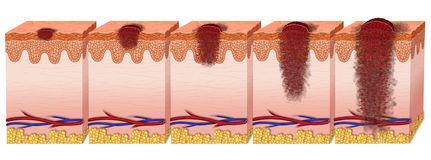
\includegraphics[scale=0.90]{figure/capitolo1/melanoma.jpg}
	\end{center}
	\caption{Melanoma}	
\end{figure}
Il melanoma cutaneo è piuttosto raro nei bambini e colpisce soprattutto attorno ai 45-50 anni, anche se l'età media alla diagnosi si è abbassata negli ultimi decenni.
\newline
In Italia, i dati AIRTUM 2017 (Associazione italiana registri tumori) stimano circa 7.300 nuovi casi ogni anno tra gli uomini e 6.700 tra le donne. L’incidenza è in continua crescita ed è addirittura raddoppiata negli ultimi 10 anni.\cite{2}
\newline
È opportuno ricordare che il melanoma cutaneo rappresenta solo una piccola percentuale (circa il 5 per cento) di tutti i tumori che colpiscono la pelle.
\subsection{Come si forma un Melanoma}
Un \textit{melanoma} inizia nelle cellule della pelle chiamate melanociti. I melanociti sono le cellule che producono la melanina, che conferisce alla pelle il suo colore. La melanina protegge anche gli strati più profondi della pelle dai dannosi raggi ultravioletti (UV) del sole. Quando le persone sono esposte alla luce del sole, i melanociti producono più melanina e inducono la pelle ad abbronzarsi, questo accade anche quando la pelle è esposta ad altre forme di luce ultravioletta (come in una cabina abbronzante). 
\newline
Se la pelle riceve la luce ultravioletta, i melanociti possono iniziare a crescere in modo anomalo e diventare cancerogeni. Questa condizione chiamata melanoma, come mostrato nella Figura 1.1, il cancro del melanoma cresce nello strato esterno dove i melanociti si trovano sulla pelle, quindi in una fase successiva si diffonde ad altre parti del corpo come ossa e polmoni.
\newline
Pertanto, il melanoma è letale se non rilevato nella fase iniziale; questa consapevolezza ha portato ad aumentare l'interesse delle soluzioni diagnostiche in fase iniziale.
Il problema della ricerca di soluzioni per il rilevamento del melanoma in fase iniziale diventa sempre più importante, in un periodo storico in cui il melanoma maligno sta aumentando rapidamente in tutto il mondo, anche nei paesi con tassi di incidenza storicamente bassi, e questo aumento si sta verificando a un ritmo sempre più veloce rispetto a qualsiasi altra neoplasia, le strategie basate sulla popolazione per controllare la malattia si sono concentrate principalmente sulla prevenzione primaria e sulla diagnosi precoce.
\subsection{Approcci e metodi per il riconoscimento}
Per l'identificazione dei melanomi, i dermatologi consigliano di utilizzare  la "\textit{regola ABCDE}" (A = asimmetria, B = irregolare
bordi, C = colore, D = dimensione, E = evoluzione).
\begin{itemize}
	\item A - asimmetria: metà di un nevo non corrisponde all'altra.
	\item B - bordi: i bordi sono irregolari, irregolari, dentellati o sfocati.
	\item C - colore: il colore non è lo stesso dappertutto e può includere sfumature di marrone o nero, o anche macchie di rosa, rosso, bianco o blu.
	\item D - dimensione/diametro: quando il diametro è un valore maggiore di 6 millimetri
	\item E - evoluzione: il nevo sta cambiando di dimensione, forma o colore
\end{itemize}
\begin{figure}[h]
	\begin{center}     
		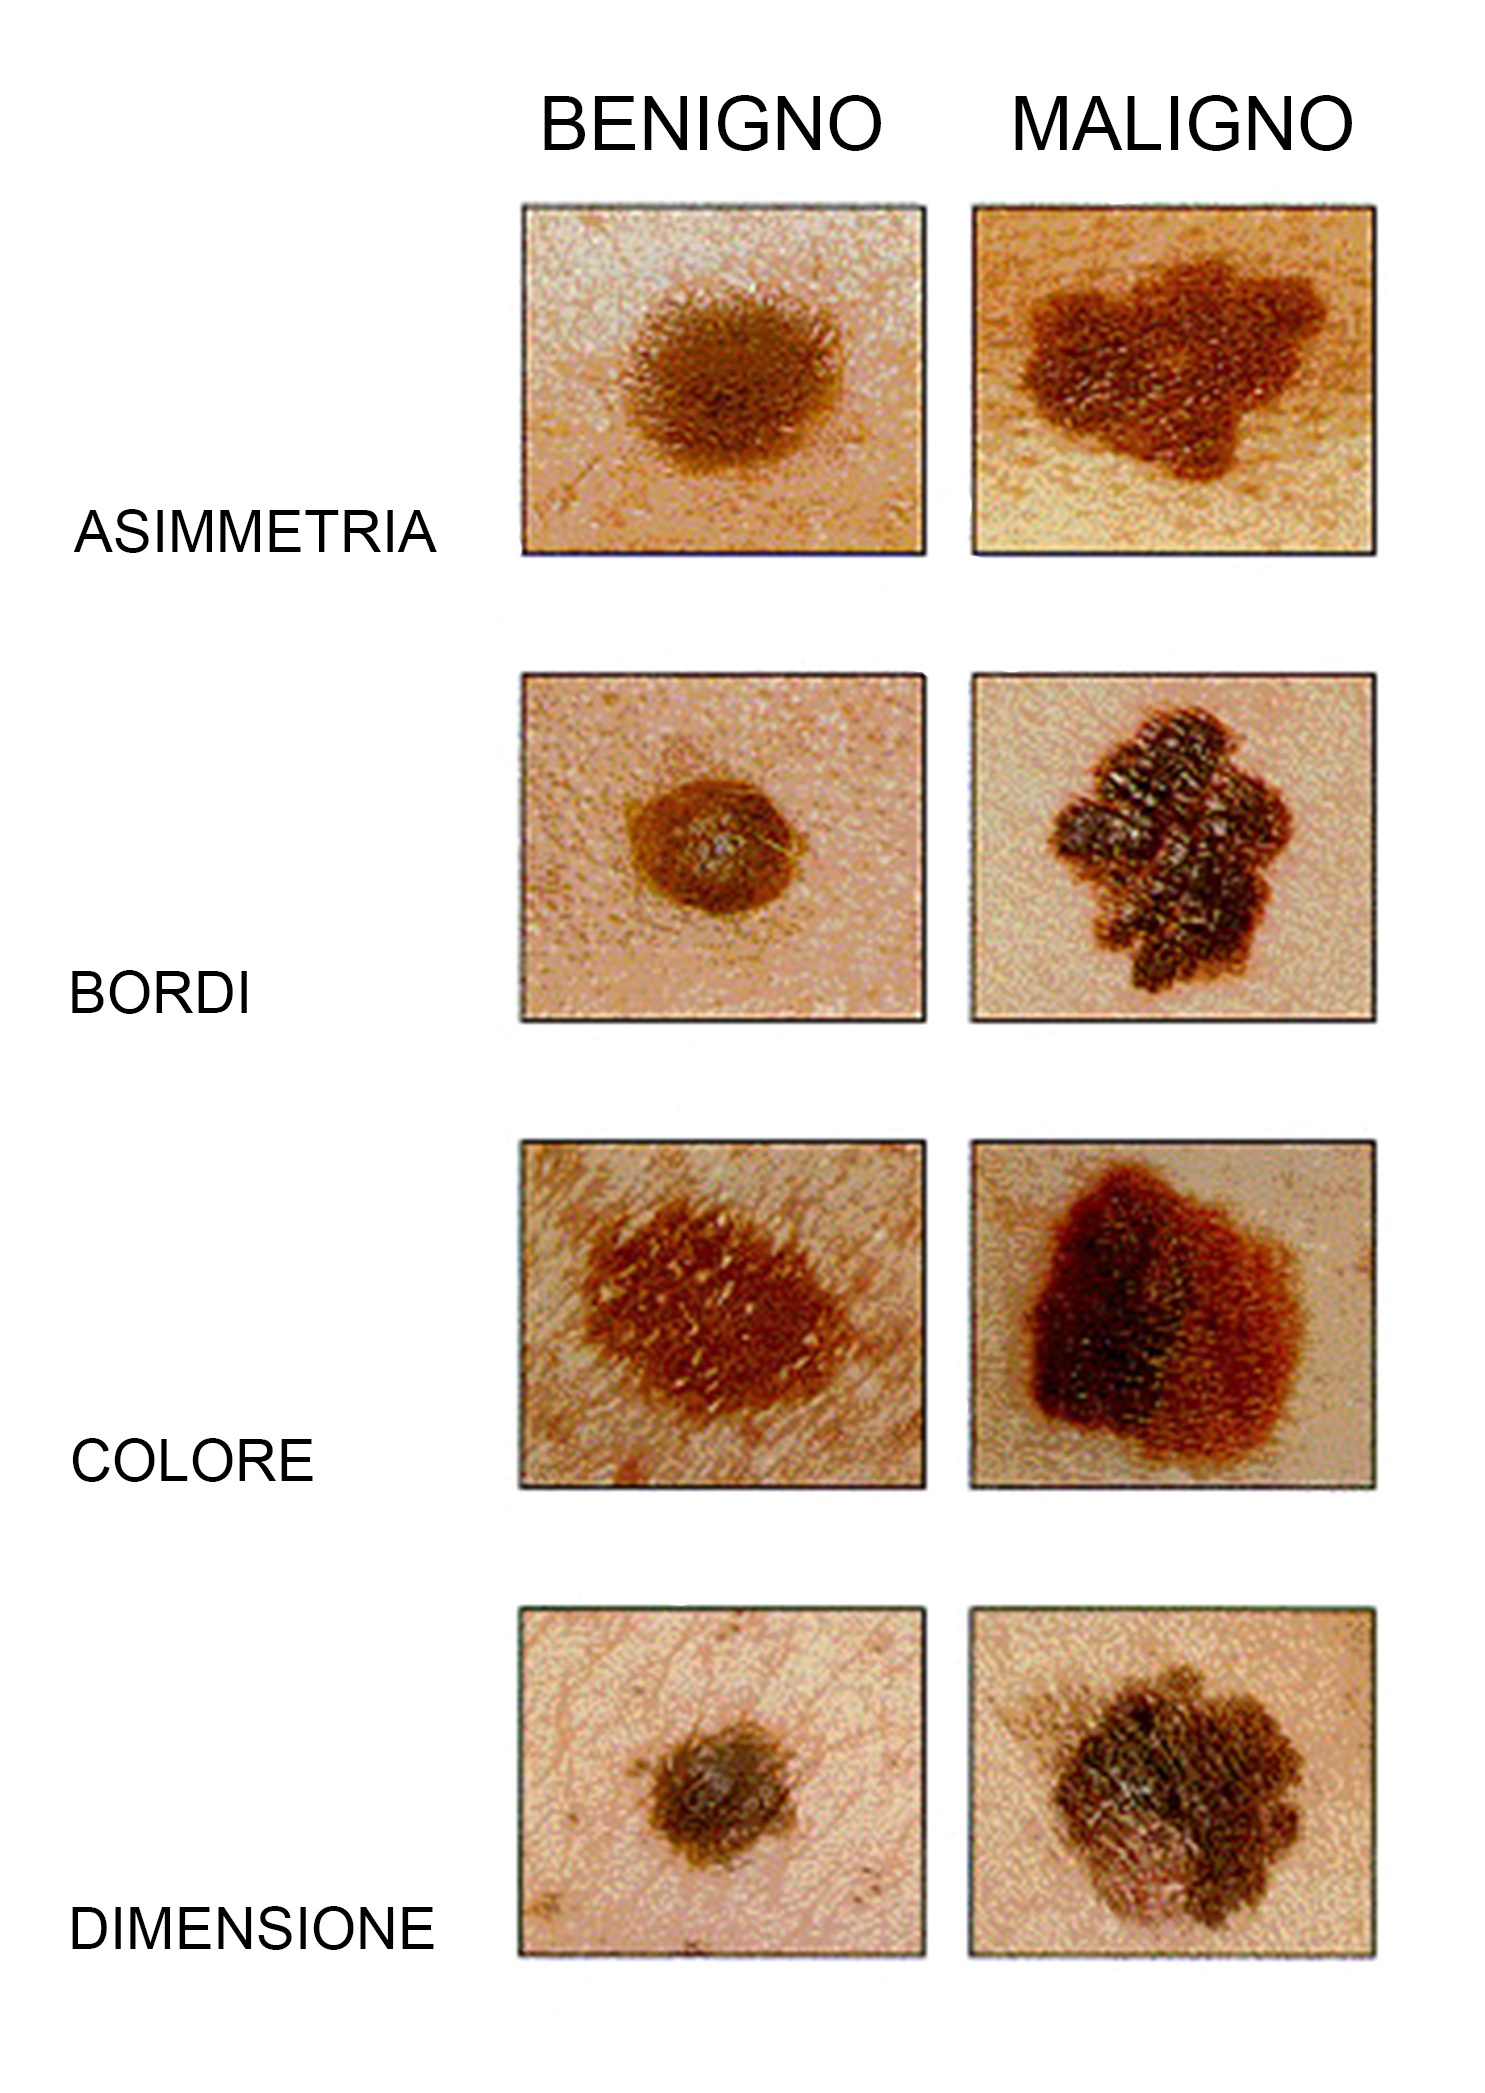
\includegraphics[scale=0.50]{figure/capitolo1/classificazione.jpg}
	\end{center}
	\caption{ABCD Features}	
\end{figure}
Il melanoma può essere confuso con altre lesioni benigne e la diagnosi differenziale si svolge osservando il colore (più intenso di
 altri nevi dello stesso soggetto), l'età di esordio (più tardi
rispetto agli altri nevi), il raddoppio della taglia in 6-8 mesi.
\newline
Forma piatta palpabile o lesione leggermente rilevata sulla pelle.
\newline
Negli ultimi vent'anni sono stati proposti sistemi di diagnosi assistita per i dermatologi, da computer basati sulla visione artificiale nella diagnosi precoce del melanoma.
 Però, questi sistemi sfruttano solo un insieme ridotto di parametri o implementano un classificatore del melanoma che cerca di sostituire i dermatologi senza supportare la loro esperienza in
classificazione delle lesioni cutanee.
\newline
L'obiettivo di questa tesi è quello di fornire al dermatologo un'assistenza all'analisi dei nevi in realtà aumentata, offrendo anche un classificatore che aiuterà il dermatologo a stabilire se il nevo può essere o meno un melanoma, ma con l'obiettivo di estrarre quante più informazioni possibili in tempo reale e visibili in realità aumentata.
\newpage
\section{Reti Neurali}
Le reti neurali sono un potente strumento utilizzato nel campo dell'intelligenza artificiale.
In realtà le reti neurali, nonostante abbiano avuto la loro esplosione negli ultimi anni, non sono per nulla recenti; il primo modello di neurone artificiale è infatti stato proposto nel 1943, negli anni successivi ci sono stati ulteriori studi e miglioramenti tra cui il modello del percettore da parte di Rosenblatt, fra gli anni '50 e gli anni '60. 
Il grande limite delle reti neurali è sempre stata la mancanza di prestazioni computazionali lato hardware che consentisse l'esecuzione di queste reti, infatti le reti neurali venivano considerate complicate e costose in termini computazionali.
\newline
L'avvento del \textit{Deep Learning} verso la fine degli anni 2000, ha portato un forte e rinnovato interesse per queste reti. \cite{maiani2016applicazioni}
\newline
\subsection{Deep Learning}
Il \textit{deep learning} è un campo di studio dell'intelligenza artificiale (AI) che consente ai sistemi di apprendere e migliorare automaticamente senza l'ausilio umano. Si concentra, in particolar modo, sullo sviluppo di applicazioni che riescono ad acquisire dati e costruire modelli che riescono a prendere decisioni in base ai dati osservati.
\newline
In base alla modalità di apprendimento adottato, i metodi di apprendimento automatico sono generalmente classificati come supervisionati o non supervisionati. Nell'apprendimento supervisionato, un modello viene costruito su determinati dati insieme alle rispettive etichette. 
\newline
Nell'apprendimento senza supervisione, invece, le etichette precedenti sono inaccessibili o accessibili ma non importanti per l'applicazione d'interesse.
Quest'ultimo, quindi, consiste nello studio di come i sistemi possano dedurre funzioni per definire strutture nascoste da dati non etichettati.
\newline
L'apprendimento semi-supervisionato è un'altra direzione il cui scopo è sfruttare i dati di un'etichetta di piccole dimensioni e dati senza etichetta di grandi dimensioni.
Uno sguardo ravvicinato alla letteratura recente direbbe che un grande focus è orientato al deep learning.
\newline
A differenza delle \textit{reti neurali tradizionali}, vari livelli di neuroni nell'apprendimento profondo eseguono un apprendimento gerarchico della rappresentazione dei dati tramite trasformazioni non lineari. In altre parole, i dati vengono passati cumulativamente attraverso una lunga catena di livelli (quindi, la descrizione profonda), dove ogni strato può essere completamente o parzialmente connesso a quello precedente.
\newpage
\subsection{Reti Neurali Convoluzionali}
Le reti neurali convoluzionali (CNN) sono di fatto delle reti neurali artificiali, ispirati a processi biologici e progettate per riconoscere modelli direttamente da immagini pixel (o altri segnali), incorporando sia l'estrazione delle caratteristiche che la classificazione.
\newline
Una tipica CNN coinvolge quattro tipi di livelli: convoluzionale, attivazione, pooling e completamente connessi (noti anche come densi). 
\newline
Uno strato convoluzionale è caratterizzato da una scarsa connettività locale, in cui ogni neurone dello strato è collegato solo ad una piccola area locale dell'input, che assomiglia al campo ricettivo nel sistema visivo umano.
\newline
I livelli di pooling riducono la sensibilità dell'output a piccoli spostamenti di input. Infine, vengono posti uno o più strati densi, ciascuno seguito da uno strato di attivazione, che producono il risultato della classificazione. La formazione delle CNN viene eseguita in modo simile a quella di altre ANN. \cite{anthimopoulos2016lung}

\section{Realtà Aumentata}
Le origini di questa tecnologia risalgono al 1901, in letteratura, in un romanzo di Frank L.Baum: "The Master Key", dove un ragazzino entra in possesso di occhiali modernissimi per l'epoca in grado di capire se le persone fossero buone o cattive attraverso una lettera\footnote{character marker} sul capo della persona che mostrava il tipo di persona.\cite{baum1901master}
\newline
\newline
La Realtà Aumentata, ad oggi, viene utilizzata in molti ambiti. Uno su tutti è lo sviluppo di applicazioni per smartphone.
\newline
Le aree di interesse della AR sono molteplici: videoludico, turistico, medico, educativo, architettonico.
\newline
La possibilità di creare oggetti virtuali in ambienti reali è di estrema utilità per la vendita di prodotti come automobili, mobili, e col tempo sta diventando un supporto sempre più richiesto in ambito medico. \cite{garofalo}

}

\chapter{Lavori correlati}
\label{cap:nomePrimoCapitoloTesi}
\lhead{\textbf{\rightmark}}

\section{Ricerche correlate}
\label{sec:nomePrimaSezioneCapitolo}
\indent{
	I riferimenti e le ricerche precedenti nella diagnosi del melanoma mobile possono essere suddivisi in tre campi:
	\begin{itemize}
		\item Miglioramento delle tecniche di rilevamento e classificazione del melanoma.
		\item Utilizzo dei dispositivi mobili nei sistemi medici e sviluppo della diagnostica assistita da computer
		\item Miglioramento dei metodi di elaborazione delle immagini per estrarre le caratteristiche del melanoma.
	\end{itemize}
	La ricerca nel primo campo determina i migliori sistemi di machine learning e tecniche di data mining, il secondo campo determina i metodi per costruire il sistema di telemedicina e le possibilità di superare la limitazione mobile nell'elaborazione e archiviazione dei dati utilizzando metodi e algoritmi commisurati alle specifiche mobili.
	\newline
	Il terzo campo è il più importante in questa ricerca, mira a trovare le tecniche di elaborazione delle immagini più accurate per catturare l'immagine e trasformarla in un insieme di funzionalità che possono essere utilizzate nella diagnosi del melanoma.
	\newline
	\newline
	Durante una visita può comparire un melanoma all'ispezione di quattro tipi:
	\newline
	\begin{enumerate}
		\item Melanoma piatto non palpabile: rappresenta la forma più frequente (70\%); tende a crescere verso l'esterno piuttosto che verso l'interno;
		\item Melanoma Cupoliforme o Nodulare: è una variante del melanoma a rapida evoluzione e ad alto rischio di progressione che tende a manifestarsi in età avanzata. Rappresenta il 10-15\% di tutti i melanomi.
		\item Lentigo Maligna (melanoma in situ): è un lento
		lesione in evoluzione che si manifesta come una macchia piatta, non palpabile, marrone, molto liscia, con perdita del normale profilo cutaneo. Generalmente ha un tasso di crescita lento (anni) e raramente si diffonde ad altre parti del corpo.
		\item Melanoma lentigginoso acrale: compare invece nelle zone acrale (palmo della mano, pianta del piede) rappresenta il 5\% di tutti i melanomi. 
	\end{enumerate}
	A causa dell'estrema eterogeneità delle lesioni, è molto difficile identificare e diagnosticare precocemente il melanoma e l'importanza di diagnosticare precocemente il melanoma non è da sottovalutare, questo perché la prognosi nel melanoma è direttamente proporzionale alla profondità della neoplasia.\cite{rigel2010evolution}
	\newline
	Nel 1985 Friedman et al. \cite{friedman1985early} proposero le regole ABCD per creare uno strumento di interpretazione diretto e semplice per i medici.
	\newline
	Successivamente, Abbasi et al. \cite{abbasi2004early} nel 2004 hanno aggiunto la lettera E (per evoluzione) come criterio di riconoscimento per il riconoscimento veloce di una lesione in evoluzione che può essere un melanoma.
	\newline
	L'efficacia del sistema ABCDE è stata convalidata in numerosi studi condotti da dermatologi \cite{carli2005diagnostic}.
	\newline
	\newline
	Le Reti Neurali (RN) rappresentano uno strumento informatico di intelligenza artificiale che ben si adatta alle problematiche clinico-diagnostiche.
	Queste sono state definite per la prima volta in ambito medico già negli anni 90.
	Lo studio di Burke et al. \cite{burke1993applicazione} del 1993, teorizza l'utilizzo delle reti neurali per la medicina di laboratorio ed in particolare per l'analisi delle cellule cancerose.
	\newline
	 Altri due principali esempi di applicazione delle reti neurali, che si trovano descritti, sono uno relativo alla diagnostica radiologica \cite{boone1990neural} e l'altro relativo all'interpretazione dei dati di laboratorio nella diagnosi dei tumori maligni del seno \cite{astion1992application}. Per quanto concerne quest'ultimo, la rete neurale era costituita da nove neuroni in ingresso, quindici neuroni intermedi, e due neuroni in uscita.
	 I nove neuroni in ingresso erano utilizzati per introdurre nella rete i valori assunti dalle nove variabili prescelte: eta' del paziente, la concentrazione nel siero del colesterolo totale, del colesterolo HDL, dei trigliceridi dell'apolipoproteina 
	A-I, dell'apolipoproteina B, dell'albumina, dell'antigene tumorale CA15-3, e l'indice di Fossel (misura dell'ampiezza delle righe dei gruppi metilene e metile nello spettro di risonanza magnetica nucleare protonica).
	 I due neuroni in uscita presentavano i valori di probabilita' (compresa tra 0 e 1) per lo stato di malattia (presenza di tumore maligno del seno) e per lo stato di non malattia (assenza di tumore maligno). 
	 La rete neurale era quindi addestrata mediante la presentazione dei dati relativi a 57 pazienti, di cui 23 con tumore maligno al seno e 34 con affezioni benigne.
	\newline
	\newline
	Per quanto concerne l'analisi dei nevi, in letteratura sono stati presentati diversi sistemi di analisi basati su applicazioni mobile.
	\newline
	Abuzaghleh, et al. \cite{abuzaghleh2014skincure}, hanno presentato un sistema basato su smartphone denominato \textit{SKIN} per assistere la diagnosi precoce del melanoma. Hanno proposto un quadro per analizzare e classificare le immagini di nevi in benigni o possibili melanomi e avvisare l'utente in tempo reale di contattare urgentemente il medico.
	\newline
	Il framework proposto ha confrontato le prestazioni di due tecniche di classificazione:
	\begin{itemize}
		\item Classificatore a un livello;
		\item Classificatore a due livelli;
	\end{itemize}
	Lo studio ha concluso che il classificatore a due livelli supera le prestazioni del classificatore a un livello.
	\newline
	Il paper però non considera alcune informazioni sulla definizione e l'estrazione di caratteristiche (Feature Extraction), ad esempio asimmetria e irregolarità dei bordi, per migliorare l'accuratezza della classificazione.
	\newline
	\newline
	Wadhawan, et al, \cite{wadhawan2011skinscan}, hanno introdotto la libreria portatile SkinScan per il rilevamento del melanoma su dispositivi portatili, una libreria implementata con C/C ++. 
	\newline
	Lo studio ha dimostrato che gli algoritmi più dispendiosi in termini di elaborazione e tempo della libreria, ovvero la segmentazione e la classificazione delle immagini, possono raggiungere una precisione e una velocità di esecuzione paragonabili a un computer desktop. Questi risultati dimostrano che è possibile eseguire applicazioni complesse di imaging biomedico su smartphone e altri dispositivi portatili, che hanno il vantaggio della portabilità.
	Ad ogni modo, il sistema richiede diverso tempo per la segmentazione e la classificazione delle immagini.
	\newline
	\newline
	Ramlakhan et al. \cite{ramlakhan2011mobile}, hanno presentato un prototipo di un sistema di riconoscimento automatizzato del melanoma basato su immagini su smartphone Android, il sistema è costituito da tre componenti principali:
	\begin{itemize}
		\item segmentazione dell'immagine
		\item estrazione delle caratteristiche basata sul metodo ABCD
		\item classificazione
	\end{itemize}
	 Il risultato sperimentale ha mostrato che il sistema non era altamente efficiente ed ha raggiunto una precisione media del 66,7\%, con una sensibilità media della classe maligna del 60,7\% e una specificità dell'80,5\%.
	 \newline
	 Il paper ha presentato due sistemi per la rilevazione di casi di melanoma nelle immagini dermoscopiche utilizzando caratteristiche di consistenza e colore.
	 \newline
	 \newline
	 Karargyris et al. \cite{karargyris2012derma}, hanno lavorato a un'applicazione mobile avanzata di elaborazione delle immagini per il monitoraggio del cancro della pelle. Gli autori hanno presentato un'applicazione per la prevenzione del melanoma, utilizzando un apparato economico (microscopio) e uno smartphone (iPhone). Questi due componenti indipendenti sono sufficienti per acquisire immagini altamente dettagliate per l'utilizzo da parte di esperti con background medico. Inoltre, un framework software avanzato per l'elaborazione delle immagini supporta il sistema per analizzare direttamente le immagini in ingresso.
	 \newline
	 L'obiettivo principale della ricerca era dimostrare come gli smartphone potrebbero trasformarsi in macchine potenti e intelligenti e aiutare grandi popolazioni senza esperienza in contesti con poche risorse. Il loro database di immagini era piccolo e consisteva di sole 6 immagini di casi normali e 6 immagini di casi sospetti.
	 \newline
	 \newline
	 Alcón et. al \cite{alcon2009automatic} hanno descritto un sistema automatico per l'ispezione delle lesioni cutanee pigmentate e la diagnosi del melanoma, che supporta le immagini delle lesioni cutanee acquisite utilizzando una fotocamera digitale convenzionale (di livello commerciale non professionale). Ancora più importante, il sistema creato include una componente di supporto decisionale, che combina il risultato della classificazione dell'immagine con la conoscenza del contesto come il tipo di pelle, l'età, il sesso e la parte del corpo interessata. Ciò consente la stima del rischio personale di melanoma, in modo da aggiungere fiducia alla classificazione. È stato verificato questo sistema classifica le immagini con una precisione dell'86\%, con una sensibilità del 94\% e una specificità del 68\%.
	 \newline
	 L'aggiunta della conoscenza del contesto è stata effettivamente in grado di indicare immagini che sono state erroneamente classificate come benigne, anche se non tutte.
	\section{Applicazioni correlate}
	Nella tecnologia e nelle applicazioni correlate, sono disponibili diverse applicazioni che offrono l'autoesame della pelle e che aiutano l'utente a classificare le lesioni cutanee in benigne o melanomi.
	\newline
	Sulla base della revisione precedente di questa applicazione \cite{wolf2013diagnostic}, le prestazioni delle applicazioni per smartphone nella valutazione del rischio di melanoma sono molto variabili e 3 delle 4 applicazioni per smartphone hanno erroneamente classificato il 30\% o più dei melanomi come benigni.
	\newline
	La revisione mostra che queste applicazioni \textbf{non sono soggette ad alcun tipo di convalida o controllo normativo.} Nonostante le dichiarazioni di non responsabilità secondo cui queste applicazioni sono destinate a scopi educativi, possono danneggiare gli utenti che potrebbero credere erroneamente che la valutazione fornita da tale applicazione sostituisce la consulenza medica. Questo rischio è di particolare preoccupazione per i pazienti economicamente svantaggiati e non assicurati (negli stati ove la sanità è privata). Poiché una percentuale sostanziale di melanomi viene rilevata inizialmente dai pazienti, il potenziale effetto di tali applicazioni sui modelli di rilevamento del melanoma è particolarmente rilevante.
	\newline
	Per queste ragioni, Freeman et al. \cite{freeman2020algorithm} nel 2020 hanno valutato la validità e le scoperte degli studi che esaminano l'accuratezza delle applicazioni per smartphone basate su algoritmi per valutare il rischio di cancro della pelle (melanoma) in lesioni cutanee sospette.
	\newline
	Sono stati inclusi nove studi che hanno valutato sei diverse app per smartphone identificabili. Sei risultati verificati utilizzando l'istologia o il follow-up (n = 725 lesioni) e tre risultati verificati utilizzando le raccomandazioni degli esperti (n = 407 lesioni). Gli studi sono risultati piccoli e di scarsa qualità metodologica, con reclutamento selettivo, alti tassi di immagini inestimabili e verifica differenziale.
	\newline
	La selezione delle lesioni e l'acquisizione delle immagini sono state eseguite dai medici piuttosto che dagli utenti di smartphone. Sono disponibili per il download due app con marchio CE (Conformit Europenne). Non è stato trovato nessuno studio peer review pubblicato sulla valutazione dell'app TeleSkin skinScan. SkinVision è stato valutato in tre studi (n = 267, 66 lesioni maligne o premaligne) e ha raggiunto una sensibilità dell'80\% (intervallo di confidenza 95\% dal 63\% al 92\%) e una specificità del 78\% (dal 67\% all'87\%) per l'individuazione di lesioni maligne o premaligne.
	\begin{figure}[h]
		\begin{center}     
			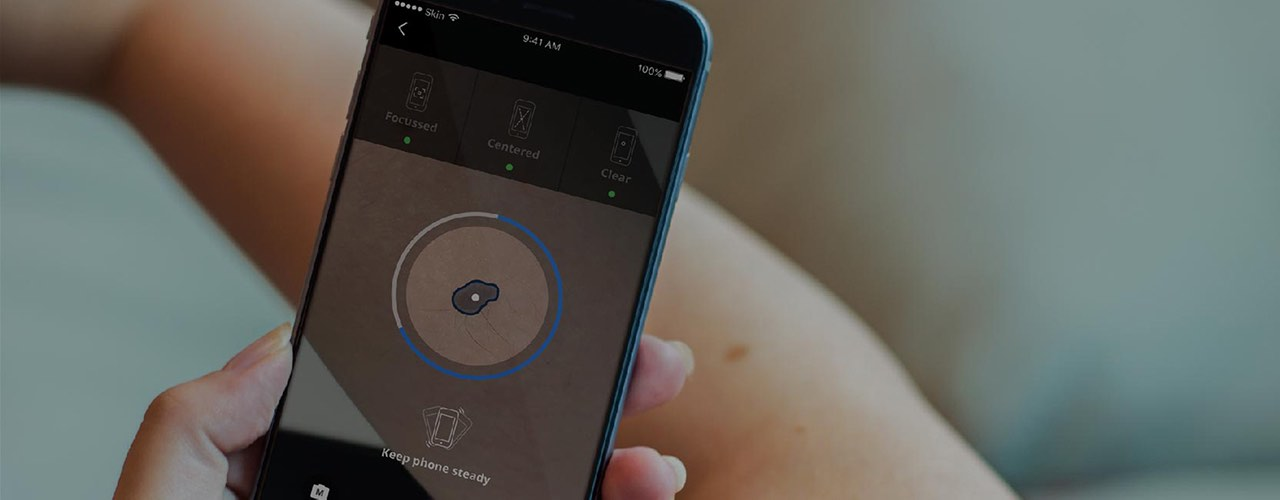
\includegraphics[scale=0.30]{figure/capitolo2/skinvision1.jpg}
		\end{center}
		\caption{Applicazione Skin Vision}	
	\end{figure}
	\newline
	La precisione dell'applicazione SkinVision verificata rispetto alle raccomandazioni degli esperti era scarsa (tre studi).
	\newline
	In conclusione non è possibile fare affidamento sulle attuali applicazioni per smartphone basate su algoritmi (spesso semplificati) per rilevare tutti i casi di melanoma o altri tumori della pelle, perché non applicabili direttamente in un ambito clinico. 
	\newline
	\newline
	Altre applicazioni esistenti sui vari application store, offrono funzionalità simili a quelle presenti in Skin Vision, tra queste è possibile annoverare:
	\newline
\textbf{Medgic} \footnote{Medgic - https://play.google.com/store/apps/details?id=co.medgic.medgic\&gl=IT}, che effettua un analisi e una valutazione ad una foto data input della cute.
	\newline
\textbf{eDerma} \footnote{eDerma - https://play.google.com/store/apps/details?id=com.thenetfirm.android.ederma\&gl=IT}, un' applicazione per il monitoraggio di lesioni cutanee che aiuta a raccogliere informazioni utili per il medico e analizzarne e comprendere l'evoluzione.
Inoltre permette al paziente di poter tenere traccia delle lesioni attraverso un sistema di fotografie passate.
	\begin{figure}[h]
	\begin{center}     
		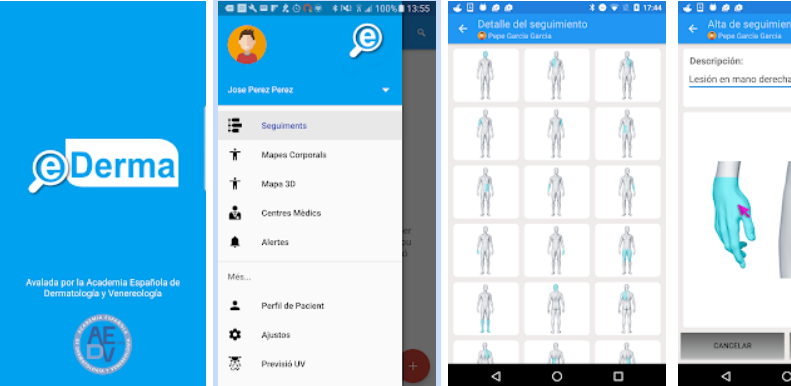
\includegraphics[scale=0.60]{figure/capitolo2/ederma.png}
	\end{center}
	\caption{Applicazione eDerma}	
\end{figure}
\newline
\textbf{Miiskin Skin Tracker} \footnote{Miiskin Skin Traker - https://apps.apple.com/us/app/miiskin-skin-tracker-ehealth/id1214795331} effettua l'imaging automatico della pelle ed utilizza algoritmi di visione artificiale coadivuati con la tecnologia di realtà aumentata per fare il confronto col tempo dei nevi analizzati in passato; questa applicazione però non effettua alcun tipo di diagnosi.
\newline
	Possiamo concludere che le applicazioni di rilevamento del melanoma esistenti presentano diverse carenze sia nell'accuratezza dei risultati sia sull'affidabilità nella diagnosi.
	\newline
	Alcune delle soluzioni proposte costituiscono un pericolo per pazienti, e anche per i dermatologi stessi, che potrebbero essere tratti in inganno dai risultati, quindi abbiamo bisogno di ulteriori ricerche per migliorare l'accuratezza.
	\newline
	Altri sistemi e soluzioni hanno dato buoni risultati in determinati dataset e contesti, ma quando si utilizzano risultati di una camera mobile abbiamo una classificazione imprecisa.
	\newline
	Questi sistemi basati su immagini ad alta risoluzione non sono sempre disponibili. 
	Altri sistemi erano corretti nella diagnosi di alcune delle caratteristiche del melanoma, ma fallivano in altro: ad esempio i risultati erano buoni nel determinare il colore della lesione, ma non riuscivano completamente a identificare proprietà come simmetria e irregolarità.
	\newline
	Attraverso una revisione dei risultati precedenti e dopo aver discusso diversi sistemi, scopriamo che 
	è necessario un lavoro di perfezionamento al fine di perfezionare l'accuratezza dei sistemi, attraverso ulteriori ricerche.
	Allo stesso tempo si può notare come la priorità sembra essere quella di rendere gli algoritmi funzionanti su dispositivi mobili invece di migliorare la precisione degli algoritmi attuali che spesso si basano su immagini raccolte con dermatoscopi professionali, e non tengono conto dell'utilizzo di altri strumenti per la cattura delle immagini di nevi.
	\newline
	\newline
	L'aspetto inerente l'utilizzo della realtà aumentata per l'analisi dei melanomi, in letteratura, ha pochi studi e ricerche, uno studio in particolare di Francese et al.  \cite{francese2020} descrive la possibilità di una applicazione in realtà aumentata che abbia lo scopo di supportare il medico nell'analisi delle lesioni del melanoma visualizzando in realtà aumentata le informazioni fornite.
	In particolare questo modello visibile in Figura prevede:
	\begin{itemize}
		\item Rilevamento della distanza.
		\item Centratura e selezione delle lesioni cutanee. 
		\item Rilevamento ottimale della luce.
		\item Classificatore CNN e parametri di funzionalità.
		\item Creazione della visualizzazione AR.
	\end{itemize}
\begin{figure}[h]
	\begin{center}
		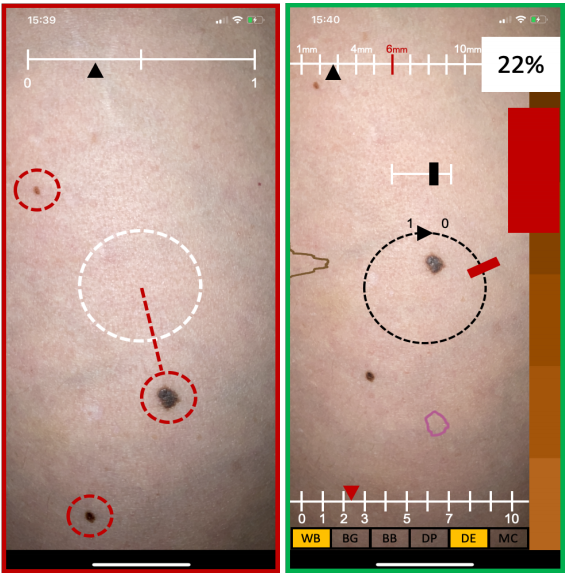
\includegraphics[scale=0.6]{figure/capitolo2/app.png}
	\end{center}
		\caption{Interfaccia proposta dallo studio di Francese et al.}	
\end{figure}
}

\chapter{Dataset HAM10000}
\label{cap:nomePrimoCapitoloTesi}
\lhead{\textbf{\rightmark}}
In questa sezione è stato descritto il dataset utilizzato per addestrare la rete neurale convoluzionale.

\section{Introduzione al Dataset}
\label{sec:nomePrimaSezioneCapitolo}

\indent{
	Il dataset HAM10000 (Human Against Machine con 10000 immagini di addestramento) è stato utilizzato in questo progetto come dataset di addestramento.
	\footnote{Il dataset HAM10000 è disponibile su Kaggle. https://www.kaggle.com/kmader/skin-cancer-mnist-ham10000/kernels} \cite{kaggle}
	Questo dataset contiene lesioni cutanee pigmentate acquisite mediante un dematoscopio standard.
	\begin{figure}[h]
		\begin{center}     
			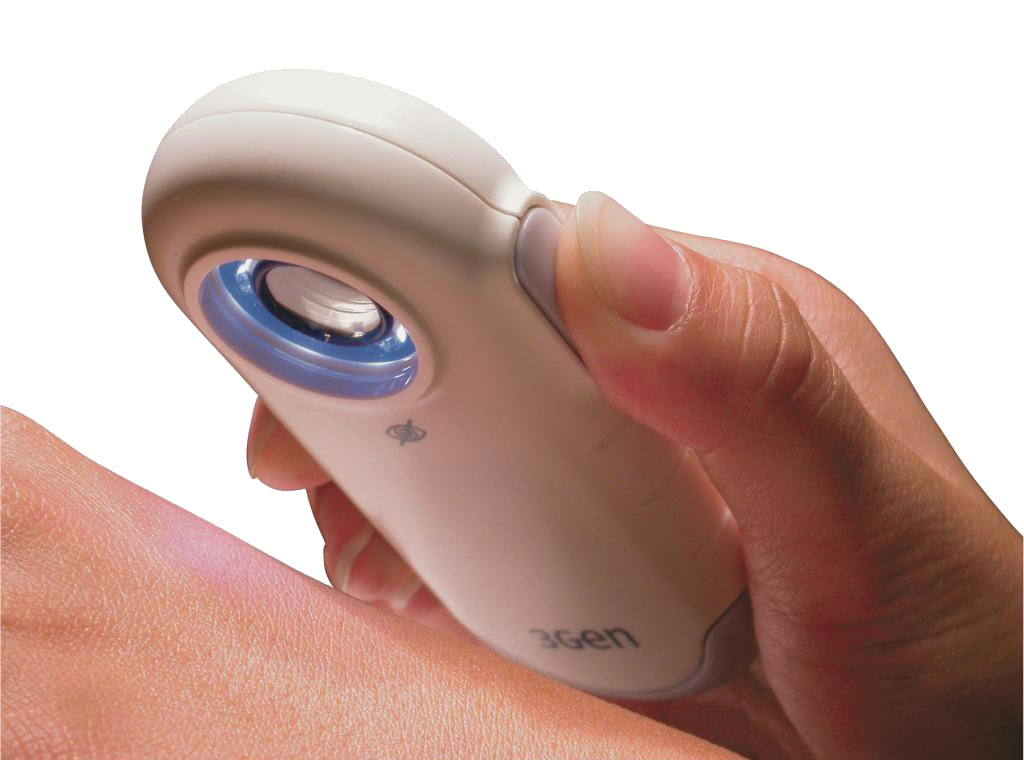
\includegraphics[scale=0.20]{figure/capitolo2/dermatoscopio.jpg}
		\end{center}
		\caption{Esempio di un dermatoscopio}	
	\end{figure}
	\newline
	\newline
	Non tutti i tipi di lesioni inizialmente studiati e sottoposti a triage attraverso la dermatoscopia sono necessariamente lesioni pigmentate. Ciò significa che, in una situazione del mondo reale, un medico generico o un infermiere che esaminano un paziente attraverso la dermatoscopia (o un paziente che esegue l'autoesame) con l'intento di presentare queste immagini a un dermatologo per un triage iniziale, potrebbero incontrare altre lesioni rispetto a quelli raffigurati in questo dataset.
	\newline
	Le lesioni classificate nel dataset HAM10000 sono: \cite{tschandl2018ham10000}
	\begin{enumerate}
		\item nv: Melanocytic nevi - neoplasie benigne dei melanociti [6705 immagini];
		\item mel: Melanoma - una neoplasia maligna derivata dai melanociti [1113 immagini]
		\item 	bkl: Cheratosi benigna - una classe generica che comprende cheratosi seborroiche, lentigo solare e lichen-planus come cheratosi [1099 immagini];
		\item cc: carcinoma basocellulare - una variante comune del carcinoma epiteliale della pelle che raramente metastatizza ma cresce in modo distruttivo se non trattata (le cc non producono necessariamente lesioni pigmentate) [514 immagini];
		\item akiec: cheratosi attinica e carcinoma intraepiteliale - varianti non invasive comuni del carcinoma a cellule squamose che possono essere trattate localmente senza chirurgia [327 immagini];
		\item vasc: lesioni cutanee vascolari che vanno dagli angiomi di ciliegia agli angiocheratomi e ai granulomi piogeni [142 immagini];
		\item df: dermatofibroma - una lesione cutanea benigna considerata come una proliferazione benigna o una reazione infiammatoria a un trauma minimo [115 immagini].
	\end{enumerate}
	
	\section{Limiti diagnostici di questo dataset}
	Le immagini dermatoscopiche da sole non forniscono dati sufficienti per una diagnosi dermatologica o un triage remoto affidabile del paziente in un ambiente di Teledermatologia.\cite{tschandl2018ham10000}
	\newline
	Le immagini dermatoscopiche mancano di contesto. Al fine di fornire un contesto, sarà necessario eseguire un protocollo di acquisizione delle immagini che includa immagini panoramiche di tutto il corpo del paziente e anche immagini di approssimazione di ciascuna lesione, che vengono acquisite con un righello o un altro quadro di riferimento visibile nell'immagine, al fine di fornire informazioni contestuali sulla dimensione della lesione. 
	\newline
	Le immagini di approssimazione scattate con il righello sono importanti anche per un paziente già in trattamento per consentire al medico assegnato di seguire l'evoluzione della lesione. Sia le immagini panoramiche che quelle di approssimazione, per essere acquisite correttamente, devono essere eseguite seguendo un protocollo che garantisca che le immagini siano a fuoco (nitide e non sfocate), prese dalla distanza corretta e con l'illuminazione corretta. \cite{von2019creating}
	Vi sono anche dettagli che non possono essere rilevati in modo affidabile attraverso la tecnica standard di dermatoscopia attualmente in uso e, in diversi casi, sarà necessaria una biopsia di conferma (noto anche come esame istologico).
	\footnote{Per un maggiore approfondimento sui protocolli di acquisizione degli esami di Teledermatologia: Aldo von Wangenheim and Daniel Holthausen Nunes. Creating a Web Infrastructure for the Support of Clinical Protocols and Clinical Management: An Example in Teledermatology. Telemedicine and e-Health. Online Ahead of Print:November 30, 2018. http://doi.org/10.1089/tmj.2018.0197. There’s also a preprint available on ResearchGate.}
	
	\section{Acquisizione immagini dermoscopiche}
	Il dermoscopio a contatto utilizzato al giorno d'oggi è il risultato di uno sforzo internazionale per la standardizzazione di questo esame effettuato durante la prima metà degli anni '90, guidato da un gruppo di ricercatori dell'Università di Monaco in Germania. Questa apparecchiatura utilizza una singola lente con un ingrandimento di 10x e un'illuminazione interna tramite LED. L'esame viene eseguito con olio minerale, che viene applicato sulla superficie della lesione prima che il dermoscopio venga applicato sulla lesione e venga scattata una fotografia.
	\begin{figure}[h]
		\begin{center}     
			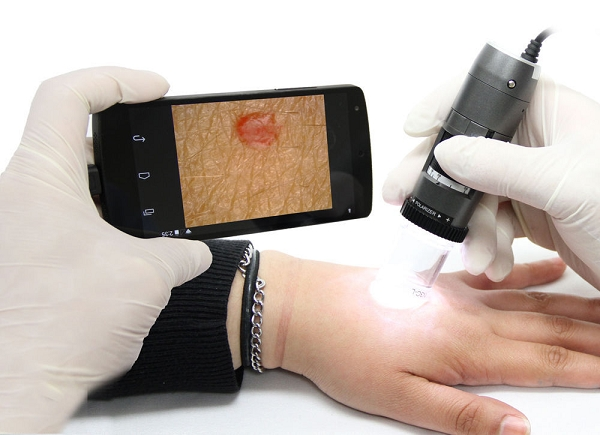
\includegraphics[scale=0.30]{figure/capitolo2/dermatoscopio.png}
		\end{center}
		\caption{Esempio a scopo illustrativo di un dermatoscopio digitale}	
	\end{figure}
	La scelta di una lente di ingrandimento monoculare 10x come standard ha consentito lo sviluppo di dispositivi molto piccoli che presto sono diventati molto popolari.
	\newline
	I dermoscopi analogici possono essere trasportati in un taschino e quelli digitali possono essere facilmente sviluppati come piccoli dispositivi USB o come adattatori per fotocamere digitali e smartphone.
	\newline
	Lo svantaggio di questo standard è che l'ingrandimento 10x non è sufficiente per il rilevamento affidabile di alcune patologie, come il carcinoma a cellule basali, che è la forma più comune di cancro della pelle. 
	\newline
	Questa forma di neoplasia è caratterizzata da alterazioni vascolari, chiamate vascolarizzazioni arboriformi, che non possono essere osservate in modo affidabile con una lente monoculare che impiega un ingrandimento 10x: sarà sempre necessaria una biopsia di conferma al fine di fornire la diagnosi definitiva.
	\newline
	Il rilevamento affidabile richiede un ingrandimento maggiore e un'ottica binoculare.
	\cite{rajpara2009systematic}

}

\chapter{Reti Neurali Convoluzionali per la Classificazione dei Melanomi}
\label{cap:nomePrimoCapitoloTesi}
\lhead{\textbf{\rightmark}}
In questo capitolo verranno presentate le reti neurali ed, in dettaglio, le reti neurali convoluzionali (note anche come CNN). Quindi sarà descritto il lavoro di addestramento della CNN e le scelte che sono state fatte in fase di progettazione.
\section{Reti Neurali Artificiali}
\label{sec:nomePrimaSezioneCapitolo}
\indent{
L'intelligenza artificiale ha contribuito in modo sostanziale a ridurre il divario tra gli esseri umani e le macchine. Una delle aree in cui l'intelligenza artificiale viene utilizzata è la Computer Vision. Una delle sfide più stimolanti è quella di consentire alle macchine di poter vedere, percepire e utilizzare conoscenza per effettuare numerose attività, tra cui la classificazione delle immagini. I progressi in campo di Computer Vision usando il Deep Learning hanno permesso di creare potenti algoritmi, tra cui le Reti Neurali. \cite{gori2003introduzione}
\newpage
Le \textbf{reti neurali artificiali (ANN)} sono modelli di calcolo matematico nati intorno agli anni ’40 del secolo scorso come riproduzione delle reti neurali biologiche. Esse svolgono funzioni di predizione ed elaborazione su insiemi estesi di dati basandosi sull’ipotesi dell’esistenza di pattern e interconnessioni fra le informazioni, costituite da neuroni artificiali, oggetto di studio.
\newline
Nella maggior parte dei casi, una rete neurale artificiale è un sistema adattivo che cambia la propria struttura in base a informazioni esterne o interne che scorrono attraverso la rete stessa durante la fase di apprendimento.
\newline
In termini pratici le reti neurali sono strutture non-lineari di dati statistici organizzate come strumenti di modellazione.
\newline
Esse possono essere utilizzate per simulare relazioni complesse tra ingressi e uscite che altre funzioni analitiche non riescono a rappresentare.
\newline
Una rete neurale artificiale riceve segnali esterni su uno strato di nodi (unità di elaborazione) d'ingresso, ciascuno dei quali è collegato con numerosi nodi interni, organizzati in più livelli. 
\newline
Ogni nodo elabora i segnali ricevuti e trasmette il risultato a nodi successivi.
\newpage
\section{Architettura delle Reti Neurali Convoluzionali}	
L'architettura delle reti neurali convoluzionali è inspirata dall'organizzazione della corteccia visiva animale,  i cui neuroni individuali sono disposti in maniera tale da rispondere alle regioni di sovrapposizione che tassellano il campo visivo. L'applicazione più popolare di una rete neurale convoluzionale è l'identificazione di cosa un'immagine rappresenta. 
\newline
Esse sono ampiamente utilizzate anche in applicazioni che processano media. 
\newline
	\begin{figure}[h]
	\begin{center}
		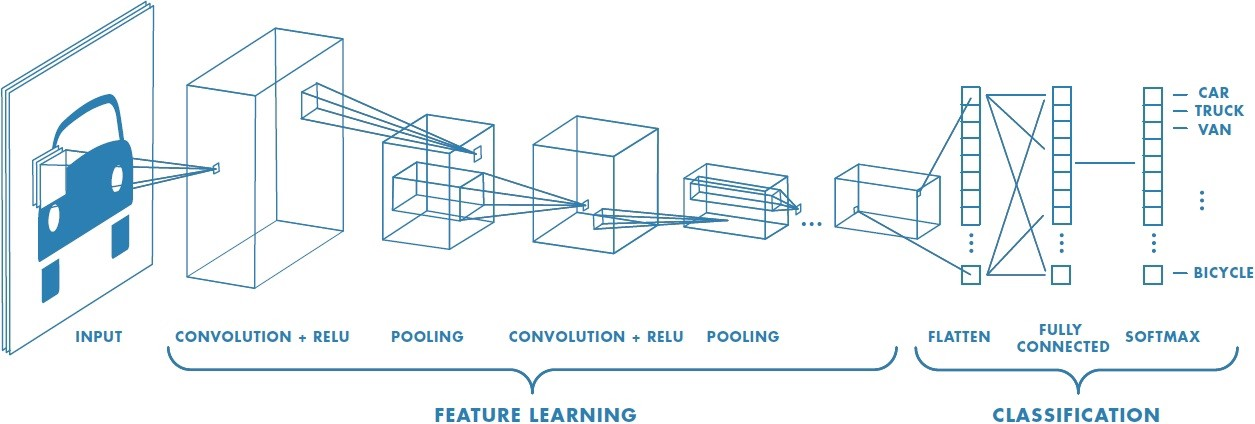
\includegraphics[scale=0.33]{figure/capitolo3/rnc.jpeg}
	\end{center}
	\caption{Esempio di costruzione CNN.}	
\end{figure}
\newline
Una Rete Neurale Convoluzionale è costituita da un blocco di input, uno o più blocchi nascosti, che effettuano calcoli tramite le funzioni di attivazione, e un blocco di output specializzato nella classificazione vera e propria. \cite{maiani2016applicazioni}
\newline
La principale differenza tra una rete neurale convoluzionale e una rete neurale classica è data dalla presenza dei livelli di convoluzione.
\newline 
L'input di una rete neurale convoluzionale è costituito da una sequenza di neuroni in grado di ricevere le informazioni dell'immagine che si vuole processare.
\newline
In questo livello, infatti, viene fornito il vettore dati che rappresenta i pixel dell'immagine in input. Nel caso di una immagine a colori RGB di dimensione 32 x 32 pixel, il vettore in ingresso avrà una dimensione 32 x 32 x 3, dove 3 rappresenta i tre colori.
\newline
Il livello convoluzionale è il principale della rete. 
\newline
L'obiettivo del livello convoluzionale è quello di individuare forme all'interno dell'immagine, come curve, linee, angoli, circonferenze o quadrati. Il livello convoluzionale fa uso di un filtro (o kernel), ossia una piccola matrice numerica che identifica una particolare struttura dell'immagine. Questa matrice si sposta sull'immagine di un determinato passo (o stride), iniziando dal punto dell'immagine in alto a sinistra.
\newline
Ogni volta che il kernel si ferma su un punto dell'immagine, dove per punto si intende la sottomatrice dell'immagine, viene calcolato il prodotto scalare tra il kernel e la sottomatrice. 
\newline
I risultati dei prodotti scalari formano l'immagine caratterizzata. Affinché l'immagine di uno strato abbia la stessa dimensione di quella dello strato precedente, è comune riempire l'immagine con zeri intorno al bordo, tale operazione viene detta \textit{zero padding}. 
\newline
Inoltre, ogni livello convoluzionale è seguito da una funzione di attivazione, la quale si pone come obiettivo quello di annullare i valori non utili dei livelli precedenti. 
\newline
La funzione di attivazione più usata è la ReLU (Rectified Linear Unit)\cite{agarap2018deep}. Questa funzione è non lineare ed è così definita: 
\begin{equation}
    f(x) = max(0,x)
\end{equation}
Un altro livello è il Pooling, che permette di ridurre l'immagine del livello convoluzionale precedente, al fine di ridurre il carico computazionale, la memoria, il numero di parametri e il rischio di Overfitting.
\newline
Il livello di Pooling usa semplicemente una funzione di aggregazione che calcola il massimo o la media dei valori dell'immagine che gli viene fornita in input.
\newline
Infine, è presente un livello FC (o Fully Connected) che effettua la classificazione vera e propria. \cite{Senn:2015}
\newpage
\section{Classificazione dei Melanomi con Deep Learning}
La metodologia utilizzata per la classificazione dei melanomi è basata su una tecnica di deep learning applicata alle immagini presenti nel dataset, in cui sono inseriti diversi tipi di malattie della pelle, inclusi i melanomi.
\newline
In particolare saranno utilizzate le reti neurali convoluzionali (CNN).
\newline
Per addestrare la CNN è stato utilizzato il dataset HAM10000.
La divisione scelta per il dataset HAM10000 consiste in:
\begin{itemize}
	\item 6705 nevi melanociti
	\item 1099 lesioni benigne
	\item 1113 melanomi
\end{itemize}
Per bilanciare i dati è stata effettuata una tecnica di data augmentation sulle immagini di melanomi.
\newline
Attraverso operazioni concatenate composte da flip orizzontali e verticali, rotazioni di 180, 90 e -90 gradi, ogni immagine originale del melanoma è stata utilizzata per generare sette immagini distinte, ottenendo così un totale di nuove 7.791 immagini che, sommate alle 1.113 iniziali, hanno formato 8.904 immagini di lesioni cutanee correlate al melanoma.
\newline
La CNN è stata addestrata con 100 epoche con un batch di 64 e utilizzando l'ottimizzatore Adam.
\newline
La rete neurale è stata costruita con 4 blocchi convoluzionali e un ultimo blocco per la classificazione. Il training set, il test set e il validation set sono stati formati considerando le percentuali 80\%, il 20\% del dataset iniziale e il 15\% del training set. 
I livelli convoluzionali utilizzano una dimensione del kernel pari a 5 e un passo di 1 e una regolarizzazione del kernel L2. 
Sono state utilizzate le Rectified Linear Units (ReLU) come funzione di attivazione per ogni livello convoluzionale e la funzione di attivazione Sigmoid nell'ultimo livello completamente connesso (FC) per avere una classificazione binaria del problema (0/1).
\begin{figure}[h]
	\begin{center}
		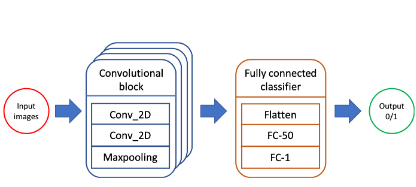
\includegraphics[scale=1]{figure/capitolo3/cnn1.png}
		\caption{CNN}	
	\end{center}
\end{figure}
\newpage
\subsection{Estrazione automatica della skin lesion}
L'estrazione automatica di una lesione cutanea in un'immagine è composta dai seguenti tre passaggi:
\begin{itemize}
	\item Hair Removal;
	\item Lesion Segmentation;
	\item Clinical Feature Segmentation;
\end{itemize}
\subsubsection{Hair Removal}
L'occlusione dei peli nelle immagini dermoscopiche influenza il funzionamento diagnostico della lesione cutanea.
Abbiamo utilizzato il rilevamento dei bordi \textbf{Canny} per la rimozione dei peli, che comprende due fasi:
\begin{itemize}
	\item nel primo, il pelo chiaro e il pelo scuro sono segmentati attraverso il rilevatore di bordi canny adattivo e la rifinitura da parte degli operatori morfologici.
	A seguito del rilevamento degli angoli di Canny, la soglia di Otsu è stata utilizzata come maschera per la rimozione dei peli al fine di ottenere un'immagine in bianco e nero. A questo punto è stato applicato un operatore di dilatazione per garantire una maggiore precisione nella cattura dei peli.
	\item Infine, è stato eseguito l'image inpainting, una tecnica che esegue una sorta di interpolazione per l'elaborazione di immagini digitali per ricostruire parti di immagini digitali danneggiate.
\end{itemize} 
\subsubsection{Lesion Segmentation}
La segmentazione mira a selezionare oggetti o regioni specifiche in una immagine sulla base di una proprietà scelta, ad esempio luminosità, colore e consistenza.
L'immagine viene convertita da RGB a scala di grigi e la parte viene separata dal suo sfondo (cioè, la pelle).
Il metodo Thresholding di TheOtsu viene utilizzato per eseguire automaticamente una soglia di immagine basata su clustering o la riduzione di un'immagine a livello di grigio in un'immagine binaria. L'algoritmo presuppone che l'immagine contenga due classi di pixel che seguono l'istogramma bimodale (cioè pixel in primo piano e pixel di sfondo); calcola quindi le soglie ottimali separando le due classi in modo che siano combinate lo spread (varianza intra-classe) è minimo. Si ipotizza che i bordi con un gradiente di intensità maggiore del valore massimo siano bordi reali, mentre quelli al di sotto del valore minimo non sono certamente bordi e quindi da scartare. 
\begin{figure}[h]
	\begin{center}
		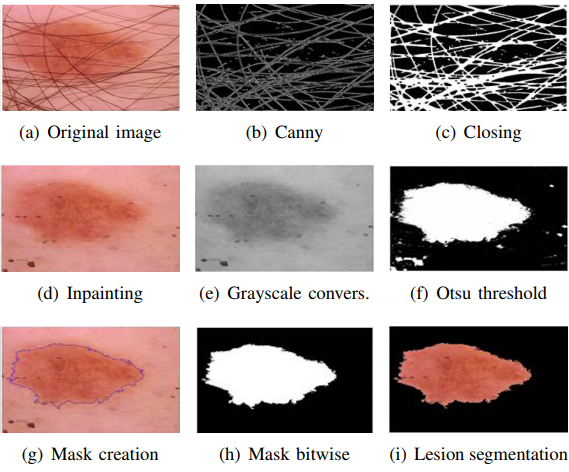
\includegraphics[scale=0.68]{figure/capitolo3/imagepro.png}
	\end{center}
	\caption{Preprocessing per ogni nevo.}	
\end{figure}
\newpage
\subsubsection{Clinical feature segmentation}
In questo caso è presente una segmentazione locale della lesione, evidenziando così le caratteristiche cliniche di una lesione come la consistenza, la forma e il colore.
\newline
Successivamente, è stato necessario ridurre l'eccessiva segmentazione, un tipico "problema" che si verifica nell'output della fase precedente. sfruttando una tecnica basata sulla media temporale e spaziale. In questo caso è stato utilizzato un filtraggio mediano che preserva i bordi rimuovendo l'eccessiva segmentazione e anche l'effetto di sfocatura.
\newline
Il filtro mediano consiste nel centrare una maschera, ordinare i pixel in modo crescente e assegnare il valore mediano al pixel del kernel.
\newline
Quindi, l'operatore AND binario bit per bit è stato applicato tra l'immagine generata e quella originale.
\newpage
\section{Addestramento}
È stata utilizzata la CNN 2D per eseguire una convoluzione spaziale bidimensionale sulle immagini. 
\newline
La CNN 2D è stata addestrata attraverso 100 epoche con una dimensione di lotto di 50 e utilizzando l'ottimizzatore Adam. 
La rete neurale è stata costruita con 4 blocchi convoluzionali (composti da strati 2D convoluzionali e Maxpool) e un ultimo blocco fully connected (FC) per la classificazione. 
\newline
Il training set, test set e validation set sono stati impostati considerando rispettivamente le percentuali 80\%, 20\% del set di dati iniziale e 20\% del training set.
\newline
I livelli convoluzionali utilizzano una dimensione del kernel di 3 e un passo di 1 e una regolarizzazione del kernel L2 per gli strati convoluzionali e densi. Sono state utilizzate le unità lineari rettificate (ReLUs) come funzione di attivazione per ogni livello convoluzionale e la funzione di attivazione sigmoide nell'ultimo livello FC per avere una classificazione binaria del problema. 
\newline
Abbiamo anche aggiunto due livelli di Dropout; uno dopo i layer Convolutional 2D e Maxpool pari a 0.25, e l'altro dopo il primo livello FC anch'esso uguale a 0.25.
}

\chapter{Metodologie}
\label{cap:nomePrimoCapitoloTesi}
\lhead{\textbf{\rightmark}}

\indent{
Il significato della diagnosi precoce del melanoma ha motivato lo sviluppo di sistemi di rilevamento/classificazione (CAD) assistiti da computer/server.
\newline 
La comunità scientifica continua a lavorare verso il miglioramento delle prestazioni diagnostiche e l'integrazione clinica della tecnologia CAD mobile.
Per questo motivo, è necessario che i sistemi CAD siano affidabili per la rilevazione/classificazione automatizzata delle lesioni del melanoma e saranno molto utili per fornire una preziosa "seconda opinione" al controllo del melanoma durante la visita dermatologica.

Dopo aver effettuato una revisione dettagliata delle tecniche e dei sistemi CAD correlati al rilevamento da smarphone o dispositivo mobile del melanoma (questa revisione includeva metodi e tecniche) si è scelto di utilizzare un approccio gerarchico (già utilizzato da altri sistemi), applicando prima passaggi di pre-elaborazione (o preprocessing) delle immagini per migliorare le strutture sospette nell'immagine e quindi impiegando l'estrazione delle caratteristiche e infine la classificazione come valutazione del nevo per indicare la presenza o meno di un melanoma. La visione delle informazioni e del livello di classificazione sarà in realtà aumentata, attraverso continous analysis e tracking del nevo.
\newline
In particolare questo lavoro si concentra sul testare ed esaminare un nuovo sistema per migliorare i seguenti aspetti:
\begin{itemize}
	\item pre-elaborazoine e miglioramento dell'immagine;
	\item pulizia dell'immagine da eventuali peli e/o imperfezioni;
	\item segmentazione accurata del nevo;
	\item feature extaction vettoriale e valutazione delle metodologie applicate per l'estrazione;
	\item visione dei risultati in realtà aumentata.
\end{itemize}
L'obiettivo finale è costruire un sistema mobile più robusto e implementarlo su un ambiente mobile/server per espandere le possibilità del sistema nell'acquisizione ed elaborazione precisa e dettagliata delle immagini.
\newline
Questo sistema faciliterà l'analisi del melanoma e fornirà la visione delle informazioni in realtà aumentata, cosicché il dermatologo o persona addetta all'analisi dei nevi potrà usufruire di un sistema robusto ed efficace ma che non va a sostituire il ruolo del medico dermatologo nell'analisi ma funge solo da supporto ad esso.
\newline
\section{Approccio proposto}
Allo stato dell'arte per la definizione dell'architettura di sviluppo in questo lavoro, ci si basa sulle attività di ricerca per l'analisi, la valutazione e il rilevamento del melanoma utilizzando la tecnologia mobile e tecniche di classificazione basate su \textit{feature extraction and classification}.\cite{mackinnon2016melanoma, taufiq2017m, chao2017smartphone, kleinjan2017introducing}
\newline
La Figura sottostante mostra l'approccio proposto.
\begin{figure}[h]
	\begin{center}
		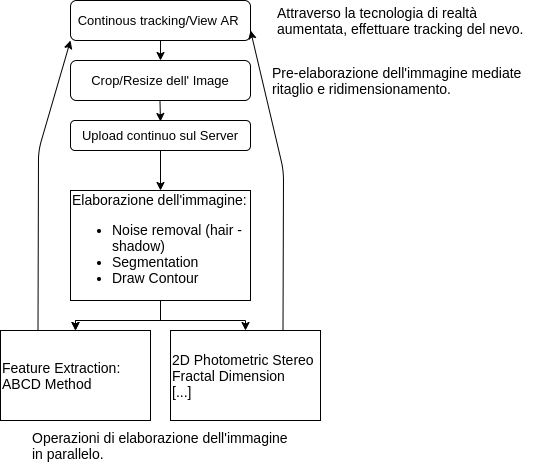
\includegraphics[scale=0.75]{figure/capitolo4/architettura.png}
	\end{center}
	\caption{Architettura di sistema ad alto livello per l'analisi dei nevi e visione in AR}	
\end{figure}
\newline
L'obiettivo di questo lavoro è testare una serie di algoritmi per il rilevamento del melanoma su un ambiente mobile/server, inviando continuamente dati ed informazioni al server; gli algoritmi di rilevamento del melanoma si basano sull'elaborazione di immagini digitali, sull'estrazione delle caratteristiche e sulle tecniche di classificazione; in questo modo sarà possibile effettuare analisi complete e visualizzare gli elementi elaborati in realtà aumentata con una latenza il più bassa possibile.
\newline
\textit{L'obiettivo ultimo è poter dare al dermatologo la possibilità di effettuare analisi di un nevo con diverse prospettive di visione garantite dalla \textbf{realtà aumentata}.}
\newline
L'approccio proposto in AR consiste nelle seguenti fasi:
\begin{enumerate}
	\item Attività di continous tracking in cui il nevo da analizzare viene in tempo reale ricercato;
	\item Taglio e ridimensionamento dell'immagine;
	\item Upload sul server;
	\item Elaborazione dell'immagine (Preprocessing);
	\item Feature Extraction:
	\subitem ABCD Method;
	\subitem 2D Photometric Stereo;
	\subitem Fractal Dimension;
	\item Valutazione del classificatore;
	\item Invio dei dati al dispositivo;
	\item Visualizzazione dei dati in Realtà Aumentata;
	\item Torna al passo 1.
\end{enumerate}
\newpage
\section{Image Preprocessing}
L'elaborazione delle immagini include molti dettagli:
\begin{enumerate}
    \item Acquisizione delle immagini utilizzando uno smartphone mobile;
    \item Pre-elaborazione delle immagini;
    \item Invio al server;
    \item Pre-processing dell'immagine (Image Pre-processing);
    \item Segmentazione;
    \item Estrazione delle caratteristiche;
\end{enumerate}
\subsection{Image Capture / Continous Tracking}
L'interfaccia di analisi deve essere semplice e pensata seguendo un approccio di utilizzo semplificato basato sui sette principi di Norman.\cite{houser1998learning}
\newline
Il \textit{continous tracking}, alla base dell'applicazione AR, permette al medico di effettuare analisi continuative sul medesimo nevo.
Il nevo dev'essere collocato al centro dell'immagine come in figura 5.2 dal dermatologo che può migliorarne la visione utilizzando il flash oppure aumentarne la dimensione attraverso lo zoom digitale.
\newpage
\subsection{Crop/Resize Image}
Prima di inviare il frame al server, questo deve essere ritagliato (crop), in modo da ridurre l'immagine e rendere il caricamento e l'analisi più veloce.
\begin{figure}[h]
	\begin{center}
		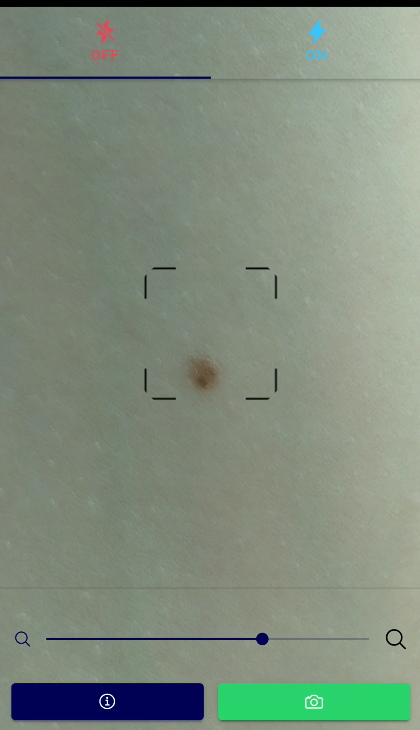
\includegraphics[scale=0.7]{figure/capitolo4/interface.png}
	\end{center}
	\caption{Esempio di interfaccia iniziale semplificata.}	
\end{figure}
\newpage
\subsection{Rimozione Peli}
Come alcune ricerche suggeriscono \cite{chatterjee2019integration, gutierrez2017skin}, il primo step del preprocessing dell'immagine per l'elaborazione di un melanoma è la rimozione dei peli dall'immagine.
\newline
Col tempo sono stati presentati diversi algoritmi e metodologie.
Poiché i frame acquisiti da smartphone includono rumore e peli, nel sistema viene utilizzata la tecnologia di riduzione del rumore in modo che i risultati della segmentazione siano ottimali.
\newline
Il problema delle ricerche precedenti sul preprocessing delle immagini con melanoma è che sono basate su immagini dermatoscopiche che sono qualitativamente e quantitativamente migliori rispetto a quelle fornite dalla fotocamera di uno smartphone.
\newline
\newline
In passato, sono state sviluppate molte tecniche per la riduzione del rumore. Una di queste è basata su filtro gaussiano. \cite{xu1999segmentation} 
\newline
Il filtro gaussiano ha però un importante difetto in quanto sfoca i bordi, e nel nostro contesto rischia di rendere imprecisa la segmentazione dei bordi. 
\newline
Pertanto, i ricercatori hanno cercato di sviluppare altre tecniche di riduzione del rumore come il filtro bilaterale per la riduzione del rumore. 
\newline
Sia I(Y) l'immagine originale e I(X) l'immagine filtrata, X e Y siano i vettori delle coordinate, e $\sigma$ è la deviazione standard della distribuzione gaussiana, quindi la riduzione del rumore utilizzando il filtro gaussiano può essere espressa come: \cite{haddad1991class,nixon2019feature}
\begin{center}
	\begin{equation}
I(X)= \frac{1}{2\pi\sigma^2 }\cdot e -\frac{x^2 + y^2}{2\sigma^2}\cdot I(Y)
	\end{equation}
\end{center}
Tuttavia, come indicato prima, il filtro gaussiano sfoca i bordi delle immagini e quindi è stato pensato di utilizzare il filtro bilaterale.
\newline
Diversamente dal filtro gaussiano, il filtro bilaterale mostra eccellenti prestazioni nella conservazione dei bordi riducendo il rumore \cite{tomasi1998bilateral}. Il filtro applicato ad immagini di nevi si rivela essere efficace in molti problemi di riduzione del rumore.
Il filtro bilaterale causa però un appiattimento dell'immagine \cite{tomasi1998bilateral} rendendo difficile l'estrazione del 2D photometric stereo in un secondo momento.
\newline
Un'alternativa che risulta essere efficace per immagini di melanomi acquisite dalla fotocamera dello smartphone è l'algoritmo proposto da H. Singh e D.O. Dantas et al.\cite{singh2019advanced, dantas2017blood}.
\newline
L'algoritmo è basato sulla creazione di una maschera a partire dall'immagine originale in gray scale ed effettua l'and tra la maschera creata con l'immagine originale.
Per ripristinare i dati persi viene utilizzato l'inpaint.(Figura 5.3).
\begin{figure}[h]
	\begin{center}
		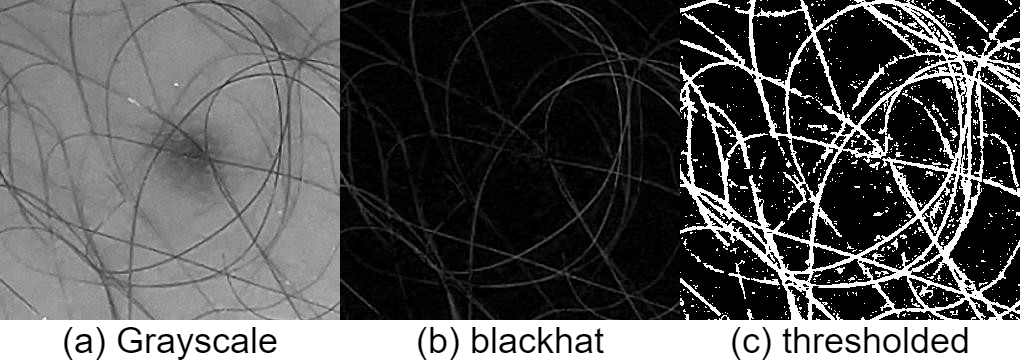
\includegraphics[scale=0.4]{figure/capitolo6/border1.png}
	\end{center}
	\caption{Preprocessing rimozione peli}	
\end{figure}
Il risultato finale è un immagine più fluida e pulita senza perdita di profondità.
\newline
\begin{figure}[h]
	\begin{center}
		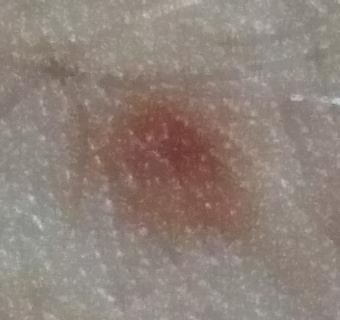
\includegraphics[scale=0.4]{figure/capitolo6/border2.jpg}
	\end{center}
	\caption{Immagine post preprocessing rimozione peli}	
\end{figure}
\newpage
\subsection{Image Segmentation}
L'obiettivo di questa elaborazione è separare il nevo dalla pelle.
\newline
La segmentazione delle immagini è una delle tecniche di base dell'image processing e della artificial vision. 
In generale, è possibile definire la segmentazione di una immagine come un processo di partizionamento del frame in gruppi omogenei, in modo tale che ciascuna regione sia omogenea ma l'unione di due regioni adiacenti non sia omogenea. \cite{haralick1985image}
\newline
Il fine ultimo della segmentazione è quello quindi di delineare i bordi del nevo, rendendo ben visibile la sua conformazione ai fini dell'analisi del dermatologo e come input per la valutazione del classificatore.  \cite{schaefer2011colour}
\newline
Nel nostro caso, la rilevazione del melanoma dipende dalle caratteristiche delle lesioni cutanee; qualsiasi errore nella segmentazione dell'immagine, per trovare il confine della lesione, può influire notevolmente sulle caratteristiche della lesione come dimensione, regolarità, rotondità e altre;.
\newline
È stato notato che nessuno degli algoritmi di segmentazione sviluppati è generalmente applicabile a tutte le immagini e diversi algoritmi non sono ugualmente adatti per particolari applicazioni.
\newline
Inoltre, la rappresentazione di un'immagine viene modificata in qualcosa che è più significativo e più facile da analizzare e facilita la selezione di una regione di interesse.
La segmentazione delle immagini è considerata il primo passo nelle applicazioni di analisi delle immagini mediche e anche uno dei compiti più critici, per questa ragione è fondamentale che le fasi precedenti abbiano processato l'immagine correttamente.
\newline
L'obiettivo della ricerca in questa fase è trovare e testare un metodo efficace e appropriato degli approcci esistenti di segmentazione delle immagini.
\newline
È stato notato che nessuno degli algoritmi di segmentazione sviluppati è generalmente applicabile a tutte le immagini e non sono ugualmente adatti per particolari applicazioni. 
\newline
Ci sono comunque molti algoritmi già sviluppati nel campo della segmentazione delle immagini, due tecniche all'avanguardia nella segmentazione delle lesioni cutanee sono state discusse in alcuni importanti lavori correlati:
\begin{itemize}
	\item Metodo di Otsu
	\item Metodo di segmentazione dello spostamento medio
\end{itemize}
\newpage
\subsubsection{Metodo della soglia di Otsu}
Se assumiamo che il confine della lesione in una certa misura sia chiaramente definito e distinto dallo sfondo, allora l'utilizzo di un semplice approccio di sogliatura come il metodo di Otsu è sufficiente per convertire l'immagine in un binario e separare la lesione dallo sfondo.
\newline
Il metodo di Otsu è un approccio non parametrico per la soglia dell'istogramma globale \cite{liu2009otsu}.
\newline
È stato sviluppato per calcolare la soglia ottimale dall'istogramma dell'immagine. Uno dei vantaggi di questo metodo è la focalizzazione su approcci non parametrici, che supportano il processo di automatizzazione del rilevamento della lesione cutanea con l'applicazione mobile senza selezione o regolazione del livello di soglia dell'utente, quindi \textbf{il metodo Otsu è uno dei migliori metodi di soglia automatica}, il principio di base nel metodo Otsu è dividere l'immagine in due classi: gli oggetti e lo sfondo.
La soglia automatica si ottiene trovando la massima
varianza tra le due classi.
L'algoritmo è il seguente:
\begin{itemize}
	\item Sia I = $[1, L]$ l'intervallo di livelli in scala di grigi dell'immagine $\phi$ (x,y) e $p_i$ la probabilità di ciascun livello
	\item Il numero di pixel con livello di grigio \textit{i} indicato con $\varphi_i$ da una probabilità di livello di grigio \textit{i} in un'immagine come $p_i=\frac{\varphi_i}{N}$
	\item La soglia automatica t che divide l'intervallo in due classi C0 = [1,..., t] e C1 = [t + 1,..., L], le distribuzioni di probabilità del livello di grigio per le due classi sono C1 e C2
	\item La media per le classi C1 e C2 sono $\mu_1$ e $\mu_2$
	\item Sia $\mu_r$ la media complessiva dell'intera immagine. Ovviamente, sommando le parti, è facile mostrare che $\mu_T$ = $\beta_1\mu_1$ + $\beta_2\mu_2$ dove $\beta_1$ = $\sum_{i=1}^{t}p_i$ e $\beta_2=$ = $\sum_{i=t+1}^{L}p_i p_i$
	\item  Dalle statistiche risulta chiaro che la somma totale delle probabilità è sempre uguale a uno $\beta_1 + \beta_2$ = 1
	\item Otsu ha definito la varianza tra classi di due classi C1 e C2 come
		\begin{equation}
		p^2=\beta_1(\mu_1 - \mu_t)^2+\beta_2(\mu_2-\mu_t)^2
		\end{equation}
	\item La soglia ottimale t è il valore che massimizza la varianza tra classi è $\sigma^2$
		\begin{equation}
		t=\max\{\sigma^2(t)\},1\leq t < L
		\end{equation}
\end{itemize}
\newpage
\subsubsection{Metodo di Segmentazione Mean Shift}
Nella sezione precedente, abbiamo ipotizzato che la lesione sia chiaramente definita e non è sempre così. Pertanto, viene proposto un algoritmo di segmentazione più accurato, chiamato \textit{clustering dei pixel}, che presenta i seguenti vantaggi:
\newline 
in primo luogo si basa sul colore dei pixel, sull'intensità e sulla posizione, o su una combinazione ponderata di questi fattori non solo sull'intensità del colore.
\newline
In secondo luogo, abbiamo più di due regioni considerate nel metodo; questo può aiutare nel caso di bordi sfocati o in presenza di rumore nella pelle.
\newline
Uno degli algoritmi di clustering più semplici è l'algoritmo K-means. 
\newline 
Il K-means è una tecnica iterativa utilizzata per partizionare un'immagine in K cluster e selezionare K cluster center, in modo casuale o in base a qualche euristica. 
\newline
L'algoritmo K-means non è appropriato per il caso studio, poiché l'obiettivo è utilizzare un algoritmo non parametrico automatizzato.
\newpage
\subsection{Estrazione del contorno}
Dopo aver segmentato l'immagine è possibile procedere ad una operazione di chiusura morfologica per rimuovere i piccoli spazi vuoti all'interno della lesione, quindi i contorni sono pronti per l'estrazione. 
\newline
"\textit{Un contorno è un elenco di punti che rappresentano, in un modo o nell'altro, una curva in un'immagine. Questa rappresentazione può essere diversa a seconda della circostanza in questione}" \cite{bradski2008learning}.
L'implementazione dell'estrazione del contorno utilizzata dalla libreria OpenCV utilizza un algoritmo che costruisce il bordo \cite{suzuki1985topological} grazie a sequenze di vertici (cioè Punti).
\newline
Il problema con questo metodo si ha quando l'immagine ha diverse sfumature di luce o ci sono più contorni selezionabili (in questo caso viene considerato il contorno più grande che non sempre contiene il nevo).
\newline
La soluzione proposta a questo problema è di filtrare le aree dei contorni, che sono più grandi di due terzi o più piccoli dei 10 pixel che quindi potrebbero essere un rumore e possono essere trascurate. 
\newline
Il seguente algoritmo viene utilizzato per selezionare il contorno della lesione dall'elenco dei contorni se il primo è maggiore di due terzi dell'intera immagine:
\begin{enumerate}
	\item Se ci sono più contorni nell'immagine, salvali in una lista
	\item Ordina i contorni nella lista e rimuovi i contorni più piccoli di 10 pixel e più larghi di 2/3 dell'immagine.
	\item Trova il massimo dei contorni
	\item Salva il contorno in una lista.
\end{enumerate}
Alla fine di questo processo è possibile disegnare il contorno sul nevo ed inoltre viene costruita un ellisse utilizzata come riferimento per le prossime analisi. Figura 5.5 (d)
	\begin{figure}[h]
	\begin{center}
		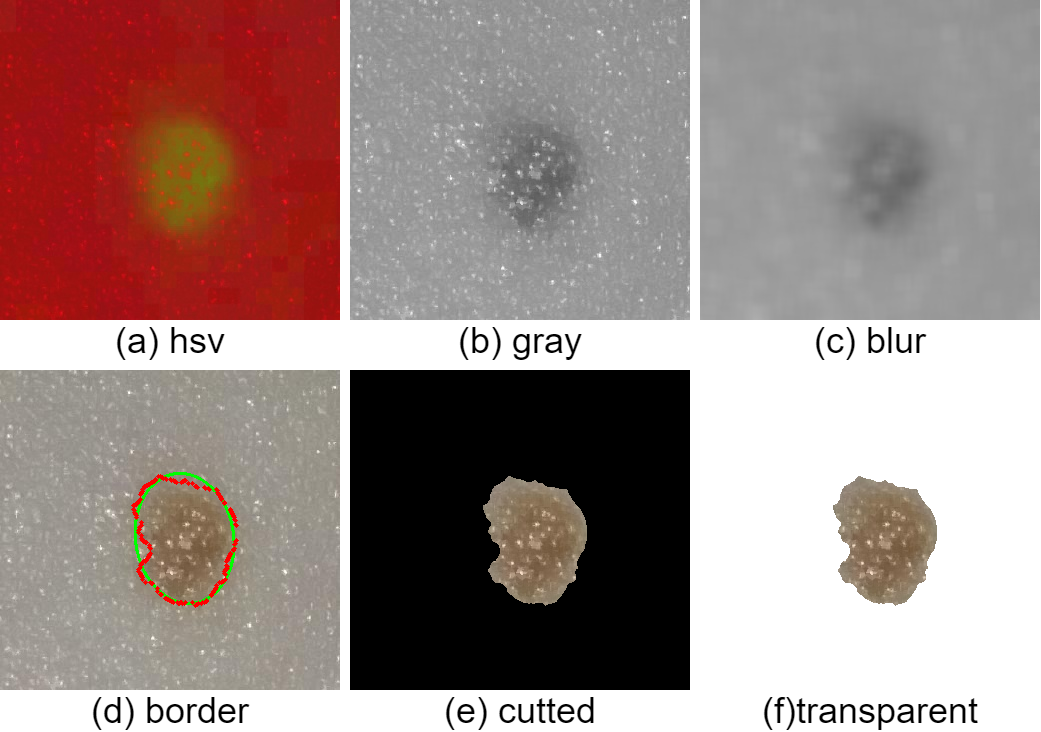
\includegraphics[scale=0.4]{figure/capitolo6/borderlist.png}
	\end{center}
	\caption{Fasi di preprocessing (Segmentazione, (a-c,e), Contorni (d))}	
\end{figure}
\subsection{Rimozione del nero}
L'ultima fase del preprocessing del nevo prima dell'estrazione delle feature e dell'analisi con il classificatore è la rimozione del nero (dato dalla segmentazione) dall'immagine.
L'algoritmo utilizzato per questa operazione è estremamente semplice:
\begin{itemize}
	\item Verifica i pixel che hanno colore nero [0, 0, 0]
	\item Converte i pixel neri in trasparenti [255, 255, 255, 0]
\end{itemize}
	\begin{figure}[h]
	\begin{center}
		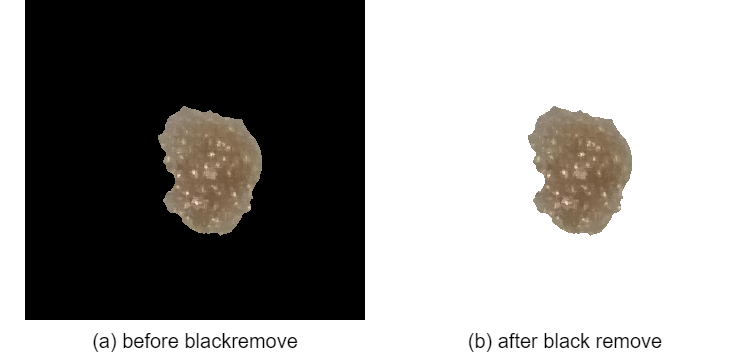
\includegraphics[scale=0.5]{figure/capitolo6/blackremove.png}
	\end{center}
	\caption{Prima e dopo l'esecuzione dell'algoritmo \textbf{black remove}}	
\end{figure}
\newpage

\section{Feature Extraction}
Dopo aver processato l'immagine correttamente è possibile procedere con l'estrazione delle caratteristiche del nevo utilizzando il metodo ABCD e aggiungendo anche altre informazioni inerenti la posizione del centroide, la visione 3D del nevo in 2D photometric stereo e la dimensione frattale. 
\subsection{Asimmetria/Simmetria}
Un nevo benigno è generalmente circolare o comunque rotondo, il melanoma è irregolare e di dimensioni maggiori; per questo motivo l'asimmetria di una lesione è di fondamentale importanza nella diagnosi. 
\newline
La lesione è generalmente contenuta in una macchia più grande. I dermatologi valutano l'asimmetria confrontando le due metà della lesione sfruttando l'asse principale come riferimento.
\newline
Per la rilevazione computazionale dell'asimmetria, esistono diversi algoritmi in letteratura.
\newline
Un possibile algoritmo per il calcolo dell'asimmetria \cite{stoecker2005detection} prevede il calcolo A=$\frac{Dist}{\sqrt{Area}}$ dove Dist è la distanza Euclidea tra il centroide e il punto più lontano, e trai il centroide della lesione fratto l'area della lesione.
\newline
In questa tesi è stato utilizzato un algoritmo che prende in input l'immagine segmentata e costruisce i contorni del nevo 4 punti di riferimento opposti tra loro, più un punto centrale (il centroide del nevo) e ne calcola il livello di asimmetria o simmetria.

\subsection{Bordo}
Per il calcolo del bordo esistono in letteratura diversi metodi.
\newline
Un riferimento principale per la valutazione del bordo è la sua circolarità.\cite{montero2009state}.
In questa attività di tesi è stato scelto di non calcolare l'irregolarità del bordo ma di lasciare al dermatologo la possibilità di visionare il contorno del nevo evidenziato di colore rosso, in modo da riuscire a vedere qualsiasi tipo di irregolarità.
\newline
Ad ogni modo analizziamo le possibile tecniche di calcolo dell'indice di irregolarità del bordo.
Uno studio di Maglogiannis et al. \cite{maglogiannis2005integrated} ha evidenziato la possibilità di calcolare l'\textbf{irregolarità del bordo} utilizzando la seguente formula:
		\begin{equation}
			Irregularity= \frac{P}{A}
		\end{equation}
Il rapporto dipende dalle dimensioni del melanoma, per questa ragione il calcolo può essere migliorato attraverso la seguente formula:
		\begin{equation}
			Irregularity= \frac{P}{Diametro Maggiore}
		\end{equation}
Un altro metodo per il calcolo dei bordi è Hull/Contour Ratio (HCR) \cite{ramlakhan2011mobile} basato sul rapporto tra il contorno dell'ellisse costruita sul melanoma ed il suo perimetro.
}
\newpage
\subsection{Colore}
Una delle prime caratteristiche di un melanoma è il colore e la varianza di colore, le lesioni da melanoma hanno infatti elementi marroni o neri in base alla produzione di melanina e al tipo di pelle.
\newline
Per questa motivazione è stato implementato un algoritmo per l'estrazione di cluster di colori \cite{faziloglu2003colour}, in questo modo il dermatologo ha la possibilità di vedere quali sono i colori che hanno una maggior presenza nel melanoma.
\newline
L'algoritmo esegue i seguenti passi:
\begin{enumerate}
	\item Prende in input un numero n (5 nel nostro caso di studio) di cluster nel quale inserire i colori.
	\item Analizza i singoli pixel del nevo ed inserisce nel cluster i pixel che hanno lo stesso colore o colore simile.
	\item Per ogni cluster costruisce un rettangolo con il colore e stampa la percentuale per ogni colore.
\end{enumerate}
Il risultato di questo algoritmo è una barra di n colori (in base al numero di cluster che si danno in input) in RGB. 
	\begin{figure}[h]
	\begin{center}
		
\includegraphics[scale=0.5]{figure/capitolo6/color.png}
	\end{center}
	\caption{Scala di colori prodotta dall'applicazione \textbf{color}}	
	\end{figure}
\newpage
\subsection{Dimensione Frattale}
Il reticolo pigmentario è un parametro di analisi molto importante, le linee della rete corrispondono alle creste epidermiche allungate e gli spazi della rete alle papille dermiche; nelle lesioni benigne, il reticolo pigmentario appare regolare e sfumato alla periferia, mentre nelle lesioni sospette appare irregolare a maglie grossolane, con pigmentazione di varia intensità, non ombreggiato alla periferia e asimmetrico.
Lo pseudoreticolo pigmentario è un'interruzione della pigmentazione da macchie ipopigmentate determinate dai follicoli piliferi e sbocchi ghiandolari. Una lesione maligna per via degli atipici melanociti aumentati di numero, appare irregolare e grossolana [4].
\newline
La dimensione frattale permette di calcolare la ripetizione di ogni sotto-struttura, questa funzione può essere fatto facilmente grazie all'analisi basata su colore analizzata in precedenza, dove ogni sotto-struttura viene inserita in un cluster.
\newpage
\subsection{Diametro}
Il melanoma tende a crescere di più dei nevi comuni, specialmente quelli con un diametro di 6 mm.
In genere, una lesione sospetta ha un diametro > 6 mm \cite{rigel2010evolution}, ma studi recenti hanno dimostrato che, con l'aumento del diametro del melanoma, aumenta anche la profondità di Breslow e che circa il 30\% delle lesioni inferiori a 6 mm sono comunque invasive.
A causa delle forme irregolari della lesione, per riuscire a calcolare il diametro viene costruito un rettangolo sull'ellisse del nevo e vengono tracciati, come riferimenti sui lati del rettangolo, il punto centrale della base e il punto centrale dell'altezza, a questo punto congiungendo i punti dei cateti paralleli si hanno diametro minimo e massimo del nevo.
\newline
Attraverso i due diametri è possibile calcolare il diametro del nevo con i seguente rapporto:
\begin{equation}
	Diametro Assoluto=\frac{dA+dB}{2}
\end{equation}
dove dA è il diametro maggiore e dB il diametro minore.
\newline
Il valore prodotto da questa funzione non è sufficiente a dare informazioni relative al nevo ma solo assolute e che dipendono fortemente dal frame dato in input; per cui, per dare una semantica alle informazioni, è necessario conoscere a che distanza si trova la camera.
\newline
Nei nuovi dispositivi dotati di sensori ad infrarossi per il calcolo della profondità il problema è di semplice risoluzione, ma con uno smartphone comune il problema è di notevole entità.
\newline
Una possibile soluzione è la divisione dei diametro dA e dB per il valore di zoom inserito per effettuare la foto, e il valore di una costante pari a 100 (Non ci sono riferimenti scientifici a sostegno di questa affermazione, ma diverse prove effettuate su nevi hanno dato risultati soddisfacenti)
\begin{equation}
	Diametro=(Diametro Assoluto/zoom)/const
\end{equation}
I passi visibili per il calcolo del diametro assoluti sono in Figura 5.8
	\begin{figure}[h]
	\begin{center}
		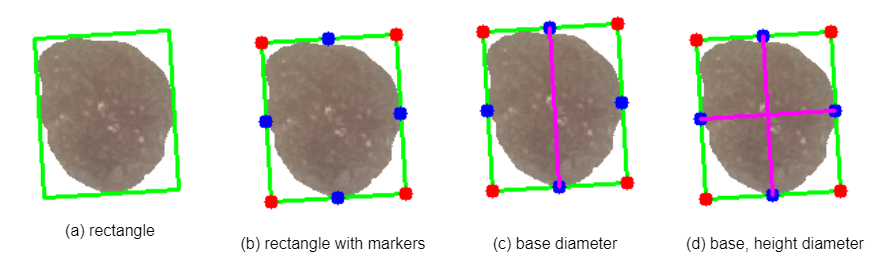
\includegraphics[scale=0.47]{figure/capitolo6/diameter.png}
	\end{center}
	\caption{Passi per il calcolo del \textbf{diametro}}	
\end{figure}
Un'altro indice utilizzabile per migliorare la precisione nel calcolo del diametro è la caratteristica focale dell'immagine, ovvero il calcolo del blur della frame, potrebbe offrire un ulteriore riferimento nel calcolo del diametro; purtroppo in letteratura non ci sono riferimenti in tal senso.
\newpage
\subsection{2D Photometric Stereo}
Un'ultima caratteristica visiva peculiare del melanoma è l'elevazione palpabile della lesione. 
\newline
Questa caratteristica viene valutata dal medico con il tatto, ma non è ancora considerata negli strumenti software, né simulata- 
\newline
La comparsa di una papula o di un nodulo nel contesto di una lesione pigmentata può spesso denotare la presenza di una lesione maligna, che è rilevabile solo palpando il melanoma.
\newline
Per questo motivo è stato adottato un algoritmo 2D photometric stereo per misurare il grado di elevazione della lesione, in maniera visiva, dando la sensazione al dermatologo di vedere in 3D il melanoma.
\newline
Il photometric stereo (utilizzato in molte applicazioni di ricostruzione 3D) è un metodo per stimare la profondità e l'orientamento della superficie di immagini, della stessa vista prese da direzioni diverse \cite{xie2016deep3d} e si basa su costruzioni normali basate sulla direzione della luce.

\textbf{Il photometric stereo} è una tecnica che stima la profondità e l'orientamento della superficie da immagini della stessa vista prese da direzioni diverse e quindi con diverse angolazioni di luce.
\newline
Teoricamente, solo tre direzioni sono sufficienti per ottenere le normali, ma per ridurre al minimo i rumori insiti nel processo, spesso è richiesto un numero superiore al minimo per immagini realistiche. \cite{verma1999photometric}
\newline
Questo metodo, tuttavia, presenta alcune limitazioni:
\begin{enumerate}
	\item La sorgente luminosa deve essere lontana dagli oggetti
	\item Macchie speculari o scure nelle regioni non danno risultati soddisfacenti
	\item le ombre devono essere mascherate per garantire una valida ricostruzione della superficie 3D.
\end{enumerate}
Il primo passo nei calcoli della normal map è calibrare la sorgente di luce, cioè stimare la direzione della luce.
\newline
Un modo per farlo è utilizzare la sfera cromata su cui viene utilizzato il punto più luminoso per identificare la direzione della luce.
\begin{figure}[h]
	\begin{center}
		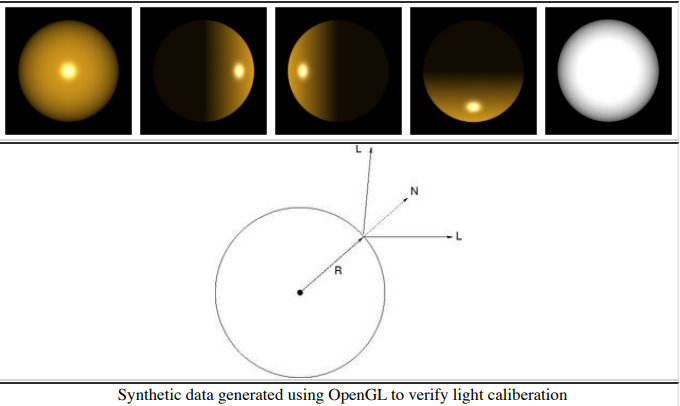
\includegraphics[scale=0.5]{figure/capitolo4/sphere.png}
	\end{center}
	\caption{Direzione della luce sulla sfera }	
\end{figure}
		\begin{equation}
		L=2(N.R)N-R
		\end{equation}
Dove R è la direzione di riflessione presa come [0,0,1]. [Px, Py] è la posizione del punto più luminoso sull'immagine e [Cx, Cy] è il centro del cromo nello spazio dell'immagine che può essere stimato dalla maskimage/.
\newline
Per le superfici Lambertain, l'intensità in qualsiasi punto della superficie può essere rilevata dall'equazione
\begin{equation}
		I=k_dN.L
\end{equation}
Dove N è la normale alla superficie ed L è la direzione della luce riflessa.
\newline
Per determinare N, abbiamo bisogno di almeno tre sorgenti luminose che non si trovano sullo stesso piano.
\newline
Pertanto, possiamo recuperare sia la mappa normale che quella dell'albedo per pixel, se il pixel riceve luce da almeno una sorgente.
\newline
Alla fine ci sono molti pixel nella regione in cui l'intensità della luce proveniente dalle sorgenti è molto bassa, quindi dobbiamo saltare quei pixel per i calcoli.
A questo punto possiamo calcolare l'immagine 3D nel nevo in 2D photometric stereo come visibile nella Figura 5.10
\newpage
\begin{figure}[h]
	\begin{center}
		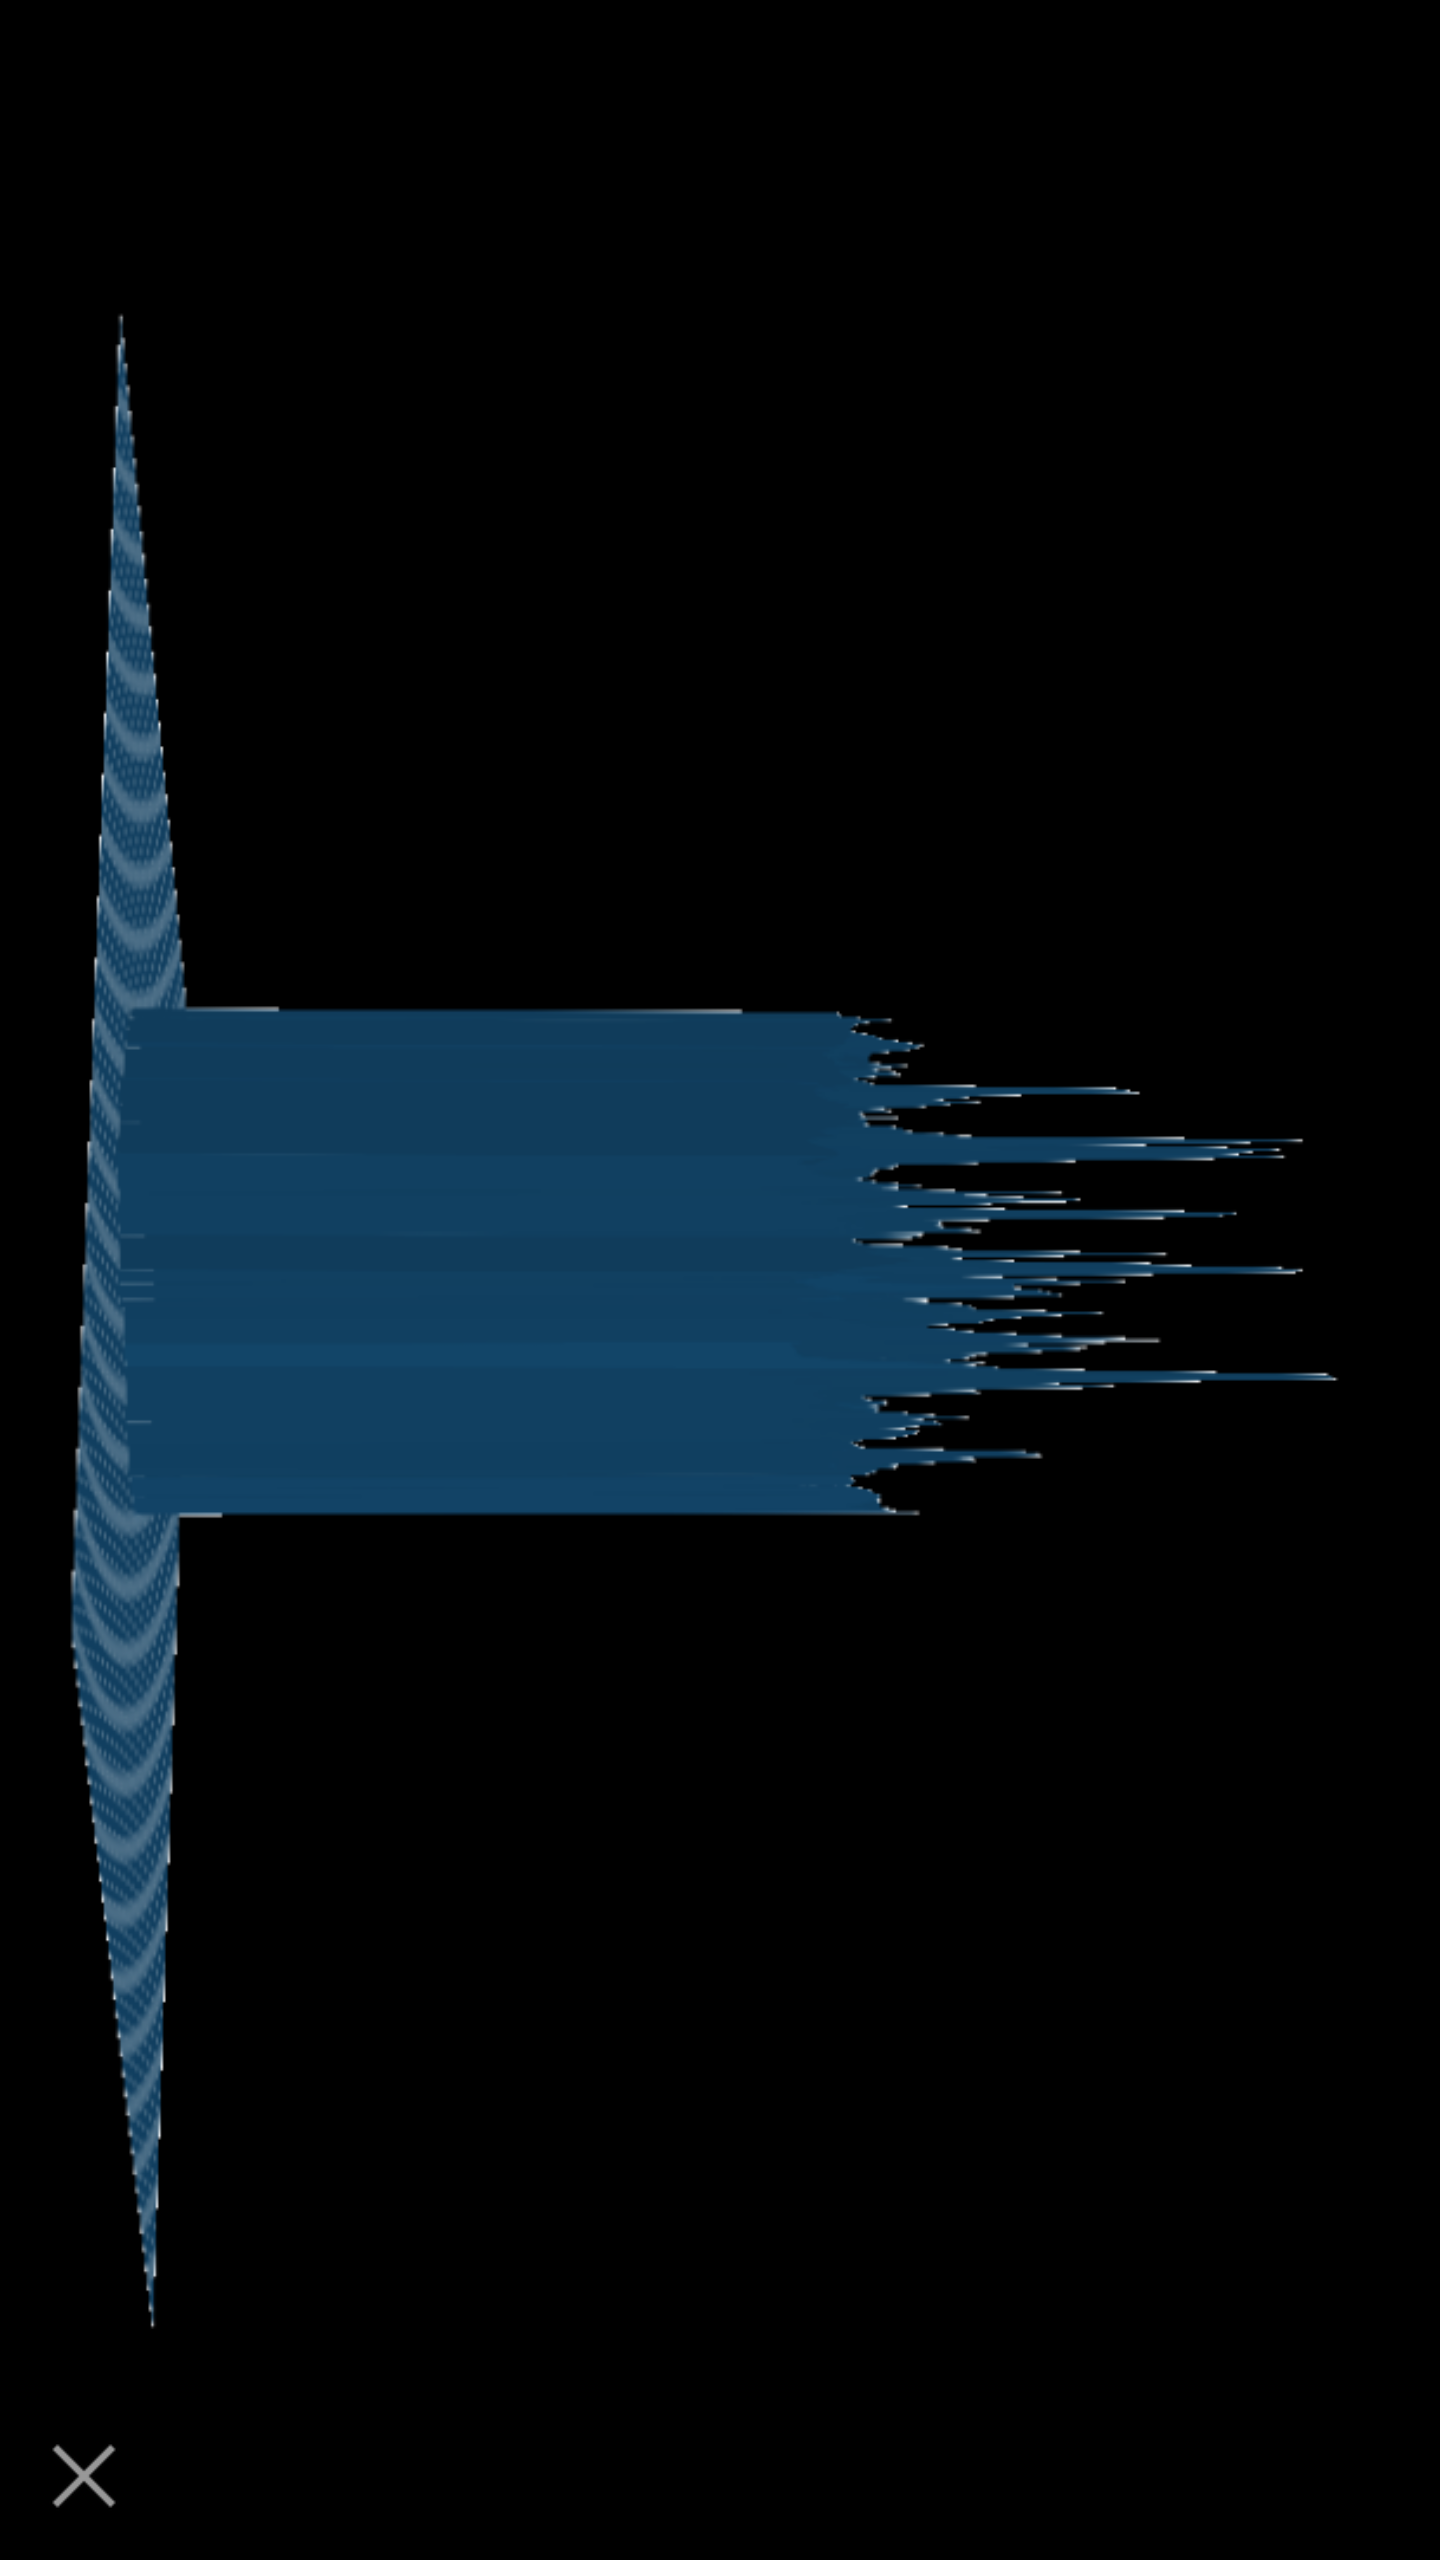
\includegraphics[scale=0.1]{figure/capitolo6/3d.png}
	\end{center}
	\caption{Immagine del nevo in \textbf{2D photometric stereo}}	
\end{figure}
\newpage
\section{Classificazione del Melanoma}
Per la classificazione e valutazione del melanoma è stato utilizzato il classificatore h5 descritto nel capitolo precedente.
L'obiettivo di questa fase è fornire al dermatologo una valutazione aggiuntiva per l'analisi del melanoma. Il classificatore è stato progettato per fornire un valore binario di valutazione con un valore di accuratezza da 0 a 1 per una migliore comprensione da parte del medico.
È stato scelto di far mostrare nell'applicazione solo il valore di accuratezza dell'analisi, poiché un valore binario avrebbe fornito una valutazione troppo approssimata dell'analisi. In questo modo, in base al grado di fiducia fornito, il dermatologo può fornire una valutazione positiva o negativa sul nevo analizzato.
\newpage
\section{Visualizzazione in Realtà Aumentata}
L'applicazione ha lo scopo di supportare il dermatologo nell'analisi dei melanomi visualizzando in realtà aumentata le informazioni fornite dalla fase di estrazione delle caratteristiche descritta nella sezione precedente.\cite{francese2020}
Alcune delle caratteristiche che l'applicazione ha sono:
\begin{itemize}
	\item Centratura e selezione delle lesioni cutanee
	\item Visione del Classificatore CNN
	\item Aggiornamento in tempo reale delle informazioni in realtà aumentata.
\end{itemize}
Un'applicazione demo che implementa tali caratteristiche è stata creata per questo progetto di tesi, e descritta nei capitoli successivi.

\chapter{Implementazione}
\label{cap:nomePrimoCapitoloTesi}
\lhead{\textbf{\rightmark}}

\indent{
	In questo capitolo è descritta l'implementazione del modello affrontato nelle metodologie.
	\newline
	Il nome scelto per l'applicazione finale realizzata è Naevus.\footnote{Vedi Appendice A per informazioni sul nome}
	\newline
	Naevus è stata svilupatta secondo un paradigma client/server.
	L'applicazione client è stata sviluppata con il framework Ionic/angular, mentre l'applicazione server con Django/python.
	\newpage
	\section{Architettura dell'applicazione Client-Server}
Il sistema è stato costruito secondo un'architettura Two-tyer, Client-Server.
\begin{figure}[h]
	\begin{center}
		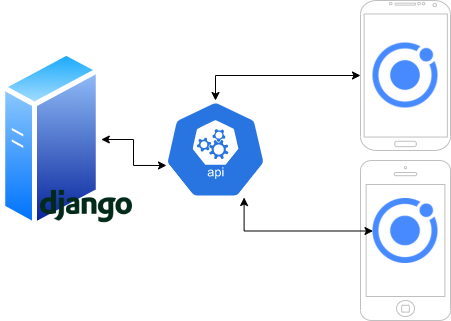
\includegraphics[scale=0.75]{figure/capitolo4/architettura1.png}
	\end{center}
	\caption{Illustrazione semplificata architettura del sistema proposto.}	
\end{figure}
\newline
L'applicazione client, sul device, presenterà all'utente i servizi di cattura dell'immagine ed i risultati dell'elaborazione avvenuta sul server con le informazioni annesse inviate tramite un metodo di comunicazione asincrono request–response; la comunicazione tra device e server avviene grazie ad un API di comunicazione presente sul device.
\begin{figure}[h]
	\begin{center}
		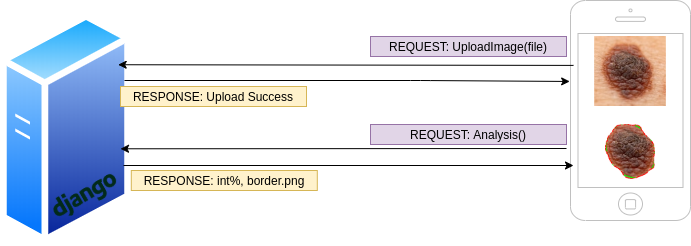
\includegraphics[scale=0.5]{figure/capitolo4/esempioarch.png}
	\end{center}
	\caption{Esempio semplificato di comunicazione Client-Server.}
\end{figure}
Per il layer di interfaccia presente sul device mobile è stato scelto il framework Ionic Angular al fine di creare un applicazione nativa cross-platform e quindi disponibile per device ios e android.
\newpage
L'architettura scelta sia per il client che per il server è stata progettata con un approccio modulare.
In questo modo l'inserimento di nuove applicazioni all'interno di django e conseguenzialmente all'interno dell'applicazione ionic è semplice e veloce, e non richiede necessariamente la conoscenza degli altri moduli che sono visti come unità blackbox.
La struttura interna di un modulo dipende in modo minimo dal “mondo esterno” e allo stesso tempo è possibile riutilizzare i moduli e svilupparli separatamente senza influenzare la struttura del codice degli altri moduli.
In questo modo se dovesse esserci un problema ad un singolo modulo gli altri non saranno influenzati (ad eccezione dell'applicazione che si occupa dell'upload dell'immagine che fornisce l'input dal quale parte l'intera analisi).
All'interno dei moduli è garantito un alto grado di modificabilità, estendibilità e di conseguenza, anche quanto detto in precedenza, è possibile aggiungere un numero indefinito di prototipi testabili anche separatamente.
\newline
Un design siffatto garantisce una low coupling – high cohesion, poiché le interazioni tra moduli sono limitate al minimo, garantendo riuso e modificabilità e di conseguenza anche manutenibilità del codice.
\newpage
\section{Sistema Proposto}
Il sistema dovrà offrire all'utente la possibilità di analizzare il nevo attraverso la camera dello smartphone ed in particolare offrire un'interfaccia di facile utilizzo e semplificata in modo da rendere gradevole e non complesso l'utilizzo dell'applicazione.
\subsection{Requisiti Funzionali}
I requisiti funzionali sono stati prodotti analizzando i lavori già esistenti e le metodologie descritte nel capitolo precedente.
\begin{itemize}
	\item \verb|RF_1| - Attiva Motore AR: Il sistema permette all'utente di attivare il motore AR per l'analisi del nevo con un click.
	\item \verb|RF_2| - Visualizza informazioni Nevo: Puntando sul nevo, il sistema inizia l'analisi del nevo.
	\item \verb|RF_3| - Visualizza Informazioni Nevo: Il sistema mostra all'utente le informazioni derivanti dall'anlisi del nevo. Le informazioni mostrate sono: asimmetria, bordo, colore, dimensione frattale, classificazione del nevo, diametro e distanza del centroide.
	\item \verb|RF_4| - Visualizza Aiuto: Il sistema permette all'utente di visualizzare la guida all'applicazione.
\end{itemize}
\newpage
\section{Design dell'applicazione client}
\subsection{AppModule}
Le applicazioni Angular possono utilizzare Cordova o Capacitor per creare app mobile native.
\newline
Nel caso specifico è stato scelto Cordova.
\newline
Per far questo è necessario importare il plug-in in @NgModule e aggiungerlo all'elenco dei provider.
\newline
Per Angular, il percorso di importazione dovrebbe terminare con /ngx. 
Il rilevamento delle modifiche di Angular viene gestito automaticamente.
Nell'applicazione Nevus progettata, sono stati utilizzati diversi plug-in al fine di fornire più funzionalità possibile lato applicazione.
I plug-in utilizzati, non standard, utilizzati nella progettazione sono:
\begin{itemize}
	\item CameraPreview da \textit{'@ionic-native/camera-preview/ngx'}:  rende disponibili le funzionalità della fotocamera per device android e ios.
	\item HttpClientModule da \textit{'@angular/common/http'}: permette l'utilizzo delle API di connessione con Django.
	\item ApiDjangoService da \textit{'./api-django.service'}: servizio creato ad hoc per la connessione con il server predisposto per l'analisi.
	\item NativeStorage da \textit{'@ionic-native/native-storage/ngx'}: permette l'utilizzo dello storage interno dell'applicazione.
	\item Base64ToGallery da \textit{'@ionic-native/base64-to-gallery/ngx';} permette il salvataggio dell'immagine scattata nella galleria del device.
	\item Crop da \textit{'@ionic-native/crop/ngx';} per il ritaglio dell'immagine scattata.
	\item PhotoViewer da \textit{'@ionic-native/photo-viewer/ngx';} permette la visione di un immagine a tutto schermo.
	\item File da \textit{'@ionic-native/file/ngx'} permette la creazione di file.
	\item Screenshot da \textit{'@ionic-native/screenshot/ngx'} permette di salvare schermate dell'applicazione.
\end{itemize}
\newpage
	\subsection {Design dell'Interfaccia}
Per lo sviluppo dell'interfaccia di "Naevus" sono state prese in esame applicazioni esistenti.
Tutte le applicazioni prese in esame hanno mostrato un numero notevole di interazioni tra applicazione e utente.
Per garantire la miglior usabilità possibile, Naevus è stata progettata in modo da garantire le  10 euristiche di Nielsen \cite{nielsen2005ten}, offrendo così un interfaccia semplice ed un estetica minimalista, garantendo corrispondenza tra mondo reale e mondo in realtà aumentata.
\newline
Il sistema è dotato di tre tipologie di interfaccia incluse in un unica interfaccia principale:
\newline
un'interfaccia pre-analisi in cui parte il motore di riconoscimento, un'interfaccia di informazione sull'utilizzo e un interfaccia di analisi che mostra le informazioni in continuo aggiornamento in realtà aumentata.
\subsection{Interfaccia pre-analisi}
Per la creazione dell'interfaccia dell'applicazione è stata utilizzata una struttura a griglia in un'unica schermata, con 2 pulsanti, in modo da rendere semplice l'utilizzo dell'applicazione anche a persone poco pratiche con la tecnologia.
\newpage
\begin{figure}[h]
	\begin{center}
		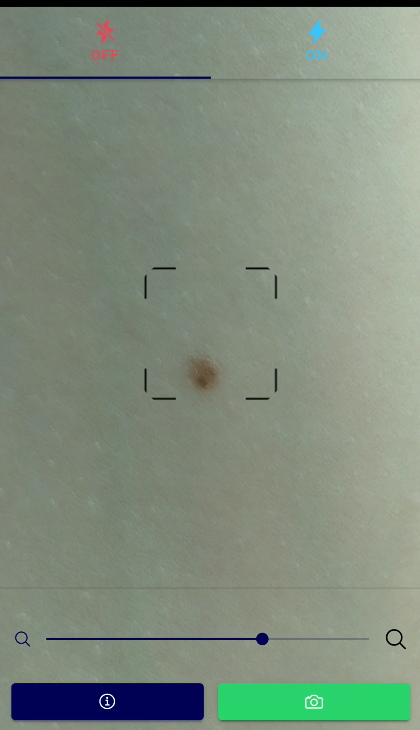
\includegraphics[scale=0.7]{figure/capitolo4/interface.png}
	\end{center}
	\caption{Schermata applicazione pre-analisi}
\end{figure}

Dall'interfaccia, visibile nella figura precedente, è possibile accendere o spegnere il flash del device ed effettuare uno zoom digitale fino a x25 \footnote{Lo zoom digitale di x25 garantisce un compromesso ideale tra zoom e qualità dell'immagine, l'aumento dello zoom troppo elevato può portare ad una perdita di qualità dell'immagine ed una difficoltà maggiore nella segmentazione del nevo da parte del server.}
\newline
Il flash è stato posizionato nell'header (in alto) dell'applicazione, in questo modo è lontano dalla zona focale situata al centro dello schermo. 
Lo zoom e il pulsante dello scatto sono stati situati in basso, in questo modo, l'utilizzo dell'applicazione può avvenire anche con una sola mano, il dermatologo o chi utilizza l'applicazione può utilizzare la mano sinistra per stabilizzare il punto ove si trova il nevo e la mano destra per scattare la foto; la medesima operazione può essere fatta anche da una persona mancina.
\newline
Prima dell'analisi è necessario far rientrare il nevo da analizzare nel mirino centrale. In questo modo l'applicazione effettuerà il ritaglio (crop) dell'immagine all'interno del mirino al fine di semplificare il lavoro del server di pulizia dei peli e segmentazione che sono onerosi.
\newpage
\subsection{Interfaccia Informazioni}
L'interfaccia informazioni offre all'utente una guida semplice ed intuitiva per l'utilizzo dell'applicazione.
\begin{figure}[h]
	\begin{center}
		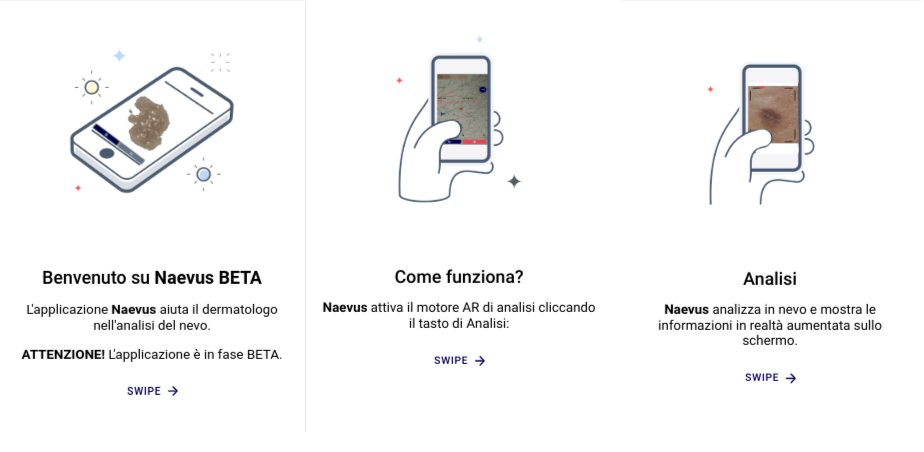
\includegraphics[scale=0.32]{figure/capitolo5/loading.png}
	\end{center}
	\caption{Schermate guida  all'applicazione}	
\end{figure}

\newpage
\subsection{Interfaccia Analisi}
L'interfaccia di Analisi in Realtà Aumentata offre all'utente la possibilità di osservare il nevo con la camera e di visualizzare le informazioni elaborate sul nevo intorno ad esso.
\begin{figure}[h]
	\begin{center}
			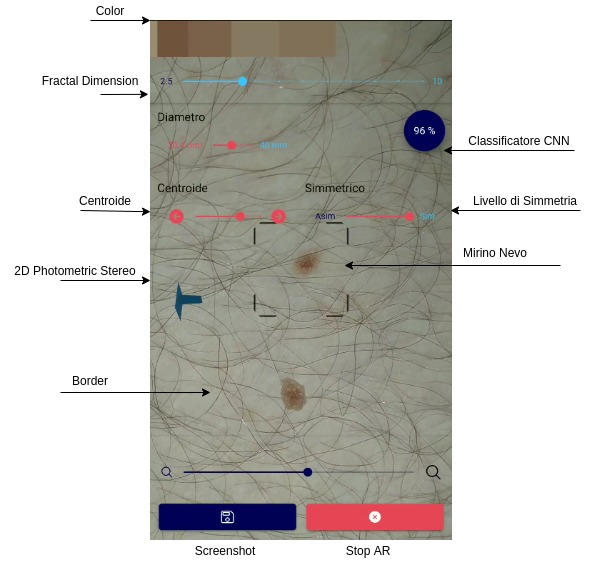
\includegraphics[scale=0.7]{figure/capitolo5/ui.jpg}
	\end{center}
	\caption{Schermate di caricamento dell'applicazione}	
\end{figure}
\newpage
Come mostrato nella figura precendente, all'interno dell'interfaccia di analisi sono presenti le caratteristiche ABCD.
All'interno dell'interfaccia è visibile, la lista dei colori assunti dal nevo sotto forma di immagine, la dimensione frattale, la dimensione del centroide, il livello di asimmetria/simmetria, la visione in 2D del nevo in modo da simulare la palpazione da parte del dermatologo, il bordo del nevo, il risultato prodotto dal classificatore H5 e la possibilità di effettuare zoom sul nevo.
Inoltre sono presenti due bottoni sul fondo, per salvare lo screenshot dell'analisi e per disattivare il motore AR.
\subsection{Photo Viewer}
Per dare la possibilità al dermatologo di visionare in dettaglio il bordo del nevo e la 2D photometric stereo, è stato implementato il plugin Photo Viewer che consente la visione a schermo pieno dell'immagine, come da esempio nella figura seguente.
Cliccando sul bordo del nevo, o sull'immagine 2D photometric stereo è possibile visionarle in alta definizione a schermo intero.
\begin{figure}[h]
	\begin{center}
		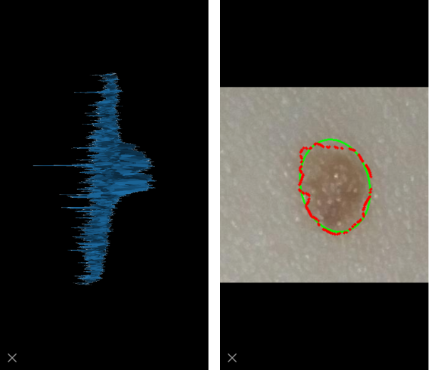
\includegraphics[scale=0.7]{figure/capitolo5/photoviewer.png}
	\end{center}
	\caption{Immagine 2D Photometric Stereo e Nevo con bordi evidenziati ed ellisse disegnata.}	
\end{figure}
\newpage
\subsection{Logica dell'interfaccia}
Per quanto concerne la logica dell'interfaccia, all'interno dei file typescript sono presenti gran parte dei comandi che consentono un utilizzo dinamico dell'interfaccia.
Le variabili sono definite prima del costruttore come da prassi fare in typescript.
\subsubsection{Camera Preview}
\textbf{CameraPreview} consente di utilizzare la fotocamera, anteriore e posteriore del device.
Viene impostato un valore base dello zoom \textit{setZoom} = 1;
Per quanto concerne la messa a fuoco dell'immagine, aspetto fondamentale di questa applicazione è stato preferito impostare una messa a fuoco semi-automatica da parte dell'utente che al click sullo schermo mette a fuoco il punto in cui si tocca oppure è la camera stessa a mettere a fuoco un oggetto che si trova al centro del mirino, in questo modo è l'utente stesso a capire se il livello di focus soddisfa o meno la visibilità del nevo;
\newline
la variabile che è stata utilizzata a tal scopo è \textit{tapfocus = false} con una impostazione semi automatica della messa a fuoco impostata tramite la variabile \textit{focusMode = 'auto';}
\newline
La Fotocamera viene attivata dal metodo \textit{async startCameraAbove()} che prova l'attivazione della camera definendo le impostazioni standard e impostando la camera posteriore (rear).
\newline
Lo scatto viene effettuato secondo impostazioni standard della fotocamera, con una risoluzione di 1280x1280 con una qualità del 100\%, senza compressione. 
\newline
L'immagine viene prima convertita in base64 e resa visibile come immagine e poi trasforamta da string base 64 a blob.
\newline
Infine il metodo \textit{base64ToGallery} permette all'app di salvare la foto appena scattata sul device.
\newline
\subsubsection{Refresh delle immagini}
Uno dei più noti problemi di ionic/angular è la difficoltà nel refresh dell'immagine quando il link di un immagine è lo stesso e l'immagine cambia, spesso ionic salva per un certo tempo le immagini di un link in cache, quindi anche quando si ricarica l'immagine; quindi anche se il refresh è attivo l'immagine viene presa dalla cache, per risolvere questo problema è stato utilizzato un trucco, ovvero un numero casuale preceduto da \textit{?} in modo da garantire il refresh anche quando si avvia una nuova analisi.
\begin{lstlisting}
...(path + "?" + (Math.random() * 3));
\end{lstlisting}
\newpage
\subsection{Servizi}
I servizi in Ionic/Angular sono dei file typescript che semplificato operazioni ricorrenti all'interno del progetto, in questo caso fungono anche da API di comunicazione con il server Django.
\subsubsection{uploading.service}
La logica di connessione per l'invio del file dal client al server è contenuta nel servizio \textbf{uploading.service.ts}.
Il servizio utilizza il plugin \textit{HttpClient} di \textit{'@angular/common/http'} e permette la comunicazione tramite richieste request-response.
\begin{lstlisting}
DJANGO_API_SERVER: string = "http://192.168.1.13:8000";
constructor(private http: HttpClient) { }

public uploadFormData(formData) {
return this.http.post<any>(`${this.DJANGO_API_SERVER}/upload/`, formData);
}
\end{lstlisting}
Quindi tramite il metodo \textit{uploadFormData} con una chiamata post viene inviata la form contenente il file da caricare. E ritorna il messaggio di successo o insuccesso dell'upload.
\subsubsection{apidjango.service}
La logica di connessione per l'invio di richieste dal client al server è contenuta nel servizio \textbf{apidjango.service.ts}.
Qui sono contenuti tutti i metodi per le chiamate alle singole applicazioni di django che si occuperanno delle analisi ed estrazioni delle caratteristiche del nevo.
In particolare:
\begin{itemize}
	\item getClassified: si occupa di lanciare la rete neurale che effettuerà l'analisi sul nevo per il riconoscimento di un melanoma.
	\item getAsymmetry: si occuapa di lanciare l'analisi per l'asimmetria del nevo e la 2D photometric stereo e torna in output un valore float.
	\item getBorder: si occupa del preprocessing e torna in output il valore del classificatore della rete neurale.
	\item getColor: si occupa dell'analisi per colore del nevo e torna in output la dimensione frattale e l'immagine dei colori.
	\item getCentroid: si occupa dell'analisi del centroid e ritorna un valore float.
	\item clearPic: si occupa della pulizia dopo l'analisi di un nevo. 
\end{itemize}
\newpage
\section{Design dell'applicazione server}
Django è un framework Web Python di alto livello che incoraggia lo sviluppo rapido e un design pulito e pragmatico ed è uno strumento gratuito e open source.
\newline
Django è stato progettato per rendere semplici e veloci le attività di sviluppo Web comuni.
Un progetto Django ha la seguente architettura,
Django ha un design standard il cui punto di forza è la possibilità di aggiungere un numero indefinito di applicazioni ed eseguirle singolarmente, in questo modo si può sfruttare al meglio il parallelismo e la possibilità di ricevere i risultati delle feature singolarmente, riducendo i tempi di analisi.
\newpage
\subsection{Struttura dell'applicazione}
L'albero dell'applicazione è strutturato nel seguente modo:
\begin{lstlisting}
backendNevus/
	manage.py
	core/
		__init__.py
		settings.py
		urls.py
		wsgi.py
		uploadapp/
	__init__.py
	admin.py
	apps.py
	models.py
	serializers.py
	tests.py
	urls.py
	views.py
border/
	[...]
	views.py
asymmetry/
	[...]
	views.py
centroid/
	[...]
	views.py
classifier/
	[...]
	views.py
color/
	[...]
	views.py
clearpic/
	[...]
	views.py
media/
\end{lstlisting}

\subsubsection{core}
Nel core dell'applicazione sono presenti gli url delle applicazioni e il collegamento alla cartella Media dove saranno salvati i file di upload ed elaborazione.
\subsection{uploadapp}
L'applicazione \textbf{uploadapp} consente l'upload da parte del dispositivo mobile, in particolare l'interfaccia visibile dall'applicazione è offerta al file \textit{views.py}:
\newpage
\subsection{Analisi del Nevo}
Nelle sezioni successive è possibile vedere come i modelli definiti nelle metodologie sono stati implementati nell'applicazione Server finale.
\newline
\subsection{border}
L'applicazione \textbf{border} si occupa del preprocessing dell'immagine caricata sul server e del ritaglio di quest'ultima, mettendo in evidenza i bordi e costruendoci sopra un ellisse che raccolga i bordi e simuli un cerchio sul nevo.
Si occupa inoltre dell'utilizzo del classificatore h5.
\subsubsection{Rimozione Peli}
Il preprocessing si occupa della pulizia dei peli dell'immagine.
Il primo procedimento è la conversione dell'immagine in grayscale, poi costruisce il kernel con un filtro morfologico, e infine vengono intensificati i peli.
\begin{figure}[h]
	\begin{center}
		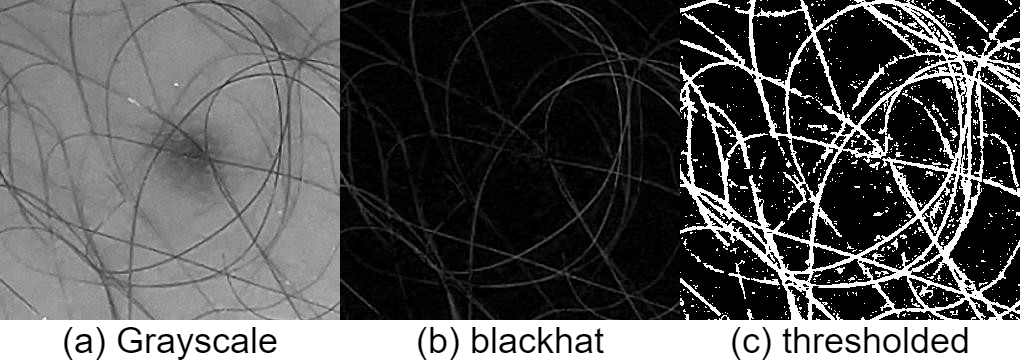
\includegraphics[scale=0.4]{figure/capitolo6/border1.png}
	\end{center}
	\caption{Preprocessing rimozione peli}	
\end{figure}
\begin{figure}[h]
	\begin{center}
		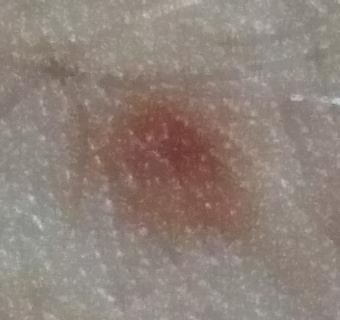
\includegraphics[scale=0.4]{figure/capitolo6/border2.jpg}
	\end{center}
	\caption{Immagine finale rimozione peli}	
\end{figure}
La scelta di inserire un valore elevato per la pulizia dei peli è dovuto alla difficoltà nei test iniziali di pulire i peli quando questi sono molto spessi e scuri. Questo scelta non influenza l'immagine priva di peli o con peli sottili ma può portare a una perdita di qualità dell'immagine quando molti peli sono sovrapposti al nevo, per cui la scelta di intensificare la rimozione dei peli ha portato una maggiore qualità quando i peli sono molto scuri come in figura 6.7; ad ogni modo si può notare che nell'immagine finale ci sono comunque tracce minime di peli come visibile in figura 6.8.
\newpage
\subsubsection{Segmentazione}
Come per la rimozione dei peli, anche per la segmentazione ho seguito un procedimento diverso rispetto a quello descritto nel Capitolo 3 di questa tesi, essendo le immagini non prodotte da un dermatoscopio digitale ma dalla camera di uno smartphone.
\newline
Le figure 6.9 da (a) a (c) mostrano le prime fasi di costruzione dell'immagine in cui viene applicato prima un filtro \textit{bgr2hsv}, in secondo luogo un filtro \textit{bgr2gray}, ed infine il \textit{blur} dell'immagine.
\newline
Infine vengono selezionati i contorni del nevo dall'immagine, e viene effettuato il ritaglio del nevo, ed in parallelo vengono evidenziati i bordi (colore rosso) e viene costruita un'ellisse a ricoprire la circonferenza del nevo (figura 6.9 (d)). 
\begin{figure}[h]
	\begin{center}
		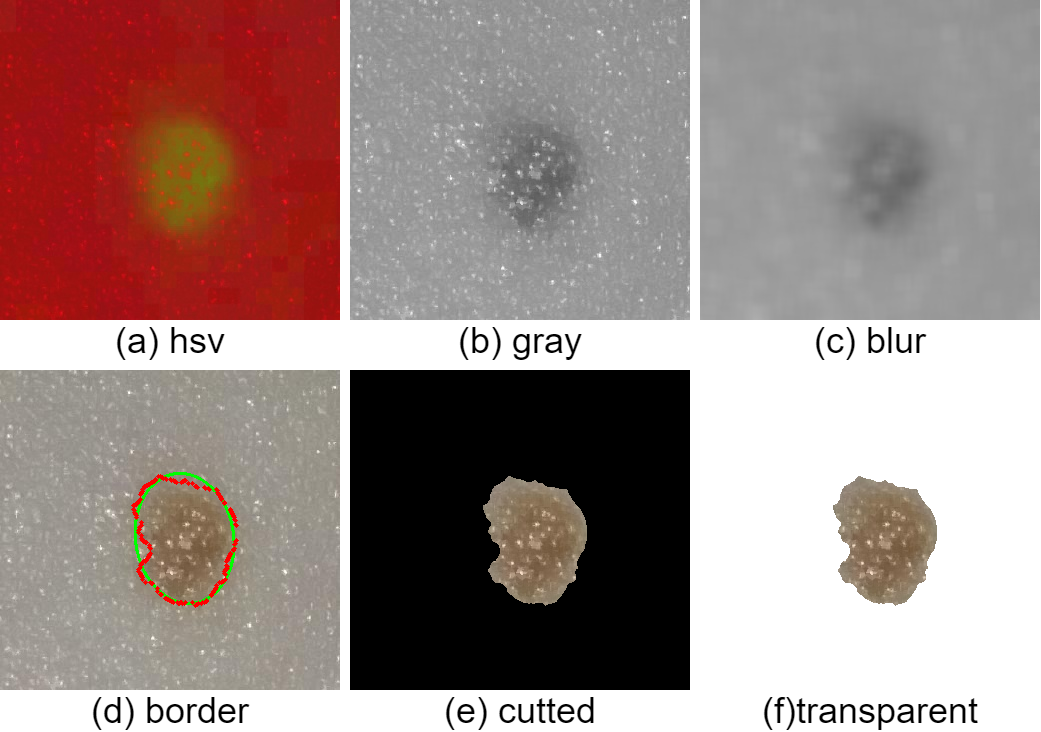
\includegraphics[scale=0.3]{figure/capitolo6/borderlist.png}
	\end{center}
	\caption{Immagine finale rimozione peli}	
\end{figure}
\newpage
\subsubsection{black remove}
L'ultima operazione richiede la rimozione del nero prodotto dalla segmentazione, per fare questo si utilizza un semplice algoritmo che trova i pixel neri e li trasforma in trasparenti; quindi il bordo viene trasformato per rendere il contorno dell'immagine trasparente (figura 6.9(e)). La trasformazione è stata fatta con il seguente algoritmo:
\begin{lstlisting}
for item in datas:
if item[0] < 3 and item[1] < 3 and item[2] < 3:
newData.append((255, 255, 255, 0))
else:
newData.append(item)
\end{lstlisting}
\begin{figure}[h]
	\begin{center}
		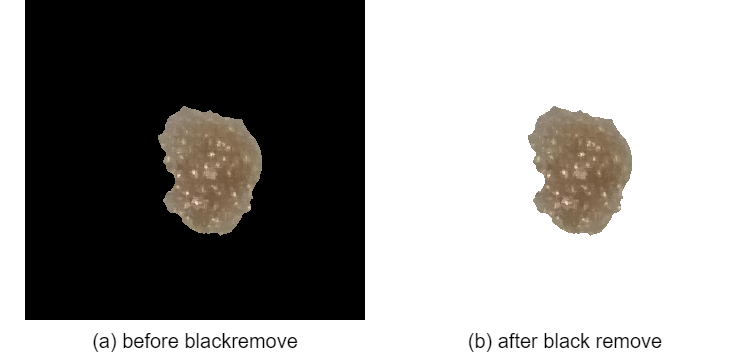
\includegraphics[scale=0.5]{figure/capitolo6/blackremove.png}
	\end{center}
	\caption{Prima e dopo l'esecuzione dell'algoritmo \textbf{black remove}}	
\end{figure}
\newpage
\subsection{asymmetry}
L'applicazione \textbf{asymmetry} calcola il livello di asimmetria del nevo e genera l'immagine 3D del nevo.
\subsubsection{asimmetria}
L'algoritmo utilizzato per calcolare l'\textbf{asimmetria} è basato sull'immagine prodotta dall'applicazione \textbf{border}.
Tramite l'ellisse che viene costruita nell'immagine in figura 6.9 (d), viene calcolata l'asimmetria del nevo. In questo modo è semplice verificare anche visivamente da parte da parte del dermatologo il livello di asimmetria.
\newline
\subsubsection{2D photometric stereo}
L'algoritmo per la trasformazione in 2D photomeric stereo prende in input l'immagine in figura 6.9(e) e la trasforma in 3D su un piano 2D.
\newpage
\subsection{classification}
Questa applicazione si occupa di calcolare la percentuale di probabilità che il nevo sia un melanoma o meno utilizzando la rete neurale convoluzionale descritta nel capitolo 3 di questa tesi.
L'immagine viene prima processata sulla dimensione per essere compatibile con il classificatore e poi data in input a quest'ultimo.
L'immagine che viene presa in input prima dell'elaborazione è quella prodotta dall'applicazione \textbf{border} figura 6.9 (e).
Il risultato dell'elaborazione (valore float da 0 a 1) viene convertito in intero ed in percentuale.
\newpage
\subsection{centroid}
L'applicazione \textbf{centroid} produce il centroide del nevo.
In valore è espresso in un range compreso tra 0 e 1 in cui 0.5 rappresenta la distanza del centroide calcolata mediante le coordinate x e y del centroide al fine di ottenere un valore compreso tra 0 e 10, se il centroide è uguale a 5 corrisponde al centro del nevo all'interno dell'ellisse.
\subsection{color}
L'applicazione \textbf{color} analizza i colori dell'immagine datagli in input e produce la percentuale di colore per ogni colore, e l'immagine con i colori più presenti all'interno dell'immagine, il numero di colori da cercare sotto forma di cluster scelto è pari a 5, questo perché un numero troppo elevato di cluster rallenta molto l'esecuzione dell'applicazione \textbf{color}.
L'immagine che prende in input color è border (figura 6.9 (e))
Il codice prevede un primo algoritmo in cui vengono indicati il numero di cluster e la chiamata a funzione che si occupa di selezionare solo i colori che hanno una percentuale minore del 70\%, questo perché altrimenti verrebbe selezionato anche il nero che fa da sfondo all'immagine.
\newline
La funzione visualize\_colors prende in input cluster e cluster.centers ed in output produce il rettangolo costruito con i cluster (di colori) che hanno percentuale inferiore al 70\% e la percentuale di colore per ogni cluster.
Se la percentuale di nero dovesse essere minore al 70\% l'immagine viene pulita da un algoritmo che analizza i singoli pixel alla ricerca del colore nero [0, 0, 0] e li rimuove dall'immagine.
L'immagine finale prodotta è presente nella figura 6.11
\begin{figure}[h]
	\begin{center}
		
\includegraphics[scale=0.5]{figure/capitolo6/color.png}
	\end{center}
	\caption{Scala di colori prodotta dall'applicazione \textbf{color}}	
\end{figure}
\newpage
\subsection{clearpic}
Clearpic è un'applicazione che mira a pulire il server dalle immagini presenti in cache, in modo da garantire un continuo e corretto funzionamento del server, dopo o prima di una analisi.
L'applicazione viene eseguita sia dal server stesso che lanciata dall'applicazione client.
Inoltre verifica la presenza dei file prodotti dall'analisi nella cartella \textit{/media} e li elimina, garantendo la possibilità di effettuare una nuova analisi.
\newpage
\subsection{diameter}
L'applicazione \textbf{diameter} prende in input l'immagine border figura 6.9 (f) e lo zoom del device e calcola il diametro del nevo.
Il calcolo del diametro richiede la trasformazione dell'immagine in gray e poi viene effettuato il blur.
Vengono costruite 4 linee intorno al nevo che costituiranno un rettangolo, dopodiché vengono costruiti 6 marker intorno al rettangolo appena costruito che saranno utilizzati per calcolare i due diametri ovvero base ed altezza del rettangolo.
Il risultato finale viene prima convertito da pollici in millimetri \footnote{1 Pollice corrisponde a 25,4 millimetri.}, ed in un secondo momento diviso per una costante pari a 100 al fine di rendere i dati significativi, infine per calcolare il diametro finale viene fatto il rapporto tra la base e l'altezza del rettangolo diviso 2.
Il risultato ottenuto è un'approssimazione del diametro, con un buon margine di errore. Nella figura sottostante è possibile notare il procedimento di analisi del nevo al fine di calcolare il diametro.
\begin{figure}[h]
	\begin{center}
		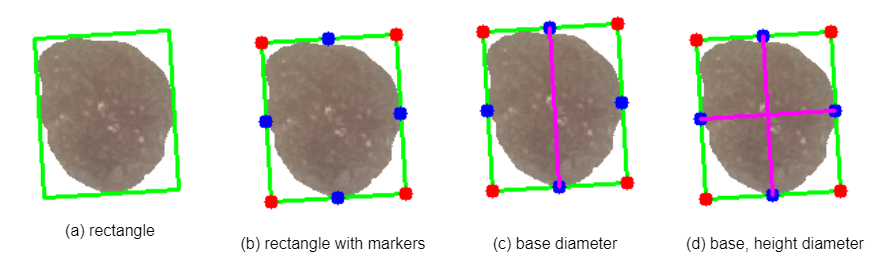
\includegraphics[scale=0.47]{figure/capitolo6/diameter.png}
			\end{center}
	\caption{Passi per il calcolo del \textbf{diametro}}	
\end{figure}

}
\chapter{Risultati e Valutazioni}
\label{cap:nomePrimoCapitoloTesi}
\lhead{\textbf{\rightmark}}

\indent{
	In questo capitolo sono presenti diverse analisi dei nevi, utilizzando l'applicazione "Naevus" e verificando se i dati sono computati correttamente e se le procedure di segmentazione e messa in evidenza dei bordi sono eseguite con successo.
	In seguito sono presentati test in diverse situazioni di luce, messa a fuoco e con presenza o meno di peli spessi o sottili.
	Saranno effettuati tre test per ogni situazione.
\newpage
\section{Analisi dei nevi }
\subsection{Analisi con luce naturale senza peli }
L'analisi del nevo con poca luce ha mostrato come sia di fondamentale importanza lanciare l'analisi in condizioni di luce ottimali se si vuole ottenere un risultato consistente e utilizzabile per il dermatologo. Il tempo impiegato per l'intera analisi sulla macchina server \footnote{vedi Appendice B} è di 5.2 secondi per frame.
\begin{figure}[h]
	\begin{center}
		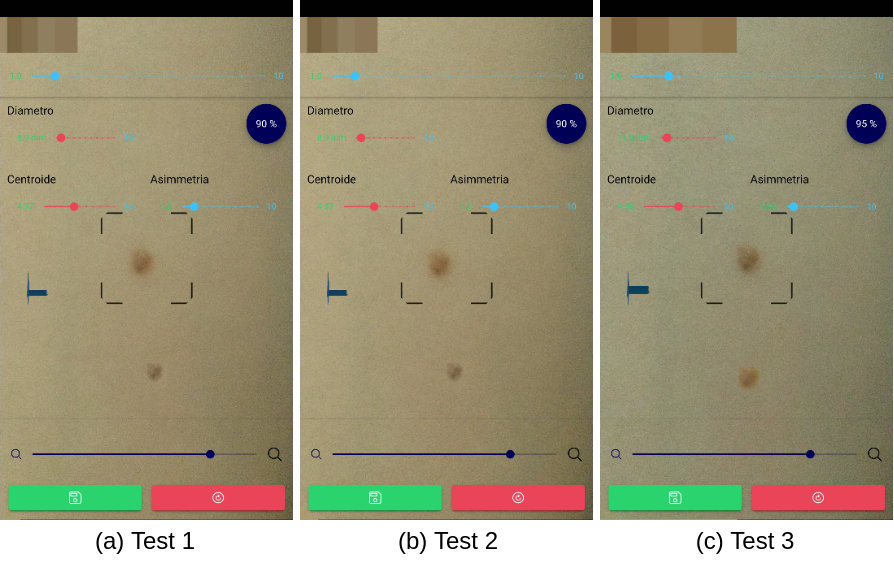
\includegraphics[scale=0.45]{figure/capitolo7/test1.png}
	\end{center}
	\caption{Analisi del nevo con poca luce}	
\end{figure}
\newpage
\subsection{Analisi con flash e luce artificiale senza peli} 
L'analisi del nevo con un livello ottimale di luce e con il flash del device acceso ha mostrato come si ottengano risultati soddisfacenti e consistenti anche in ulteriori analisi.
\newline
I risultati in Figura 7.2 sono molto simili tra di loro e discostano di pochi punti per ogni feature.
Questa analisi ha dimostrato la necessità di una buona illuminazione quando si analizza il nevo.
La media dei tempi per l'analisi è di 5 secondi. 
\begin{figure}[h]
	\begin{center}
		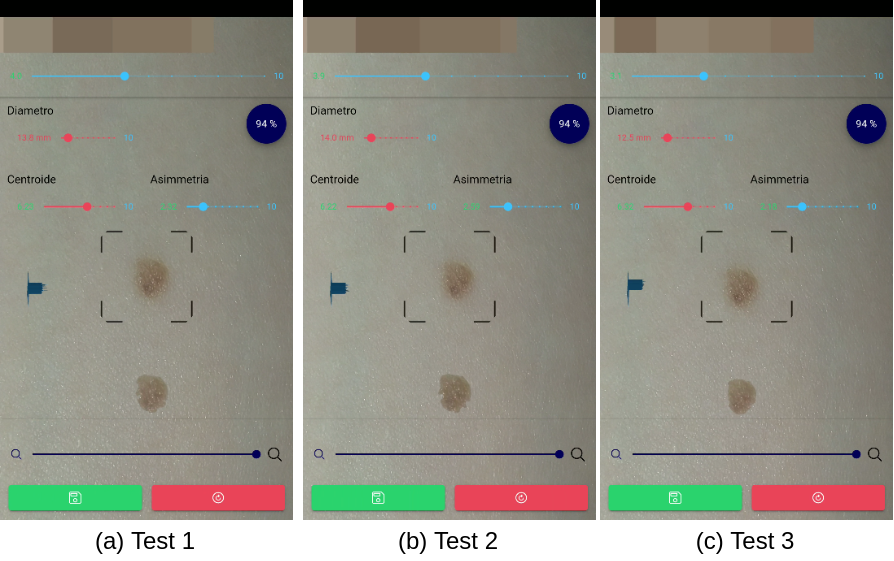
\includegraphics[scale=0.45]{figure/capitolo7/test2.png}
	\end{center}
	\caption{Analisi del nevo con flash e luce artificiale}	
\end{figure}
\newpage
\subsection{Analisi con flash e luce artificiale con peli} 
Come visto in precedenza, nel caso in cui il nevo sia coperto da peli, sarà necessario applicare l'algoritmo di \textbf{rimozione peli}.
Nella Figura 7.3 si nota che nel primo test di analisi (a) la segmentazione non è riuscita a selezionare il nevo correttamente, mentre aumentando al massimo lo zoom sul nevo nei test (b) e (c) i risultati ottenuti sono stati soddisfacenti e simili tra loro.
Il tempo impiegato per l'intera analisi sulla macchina server \footnote{vedi Appendice B} è di 6.5 secondi per frame.
\begin{figure}[h]
	\begin{center}
		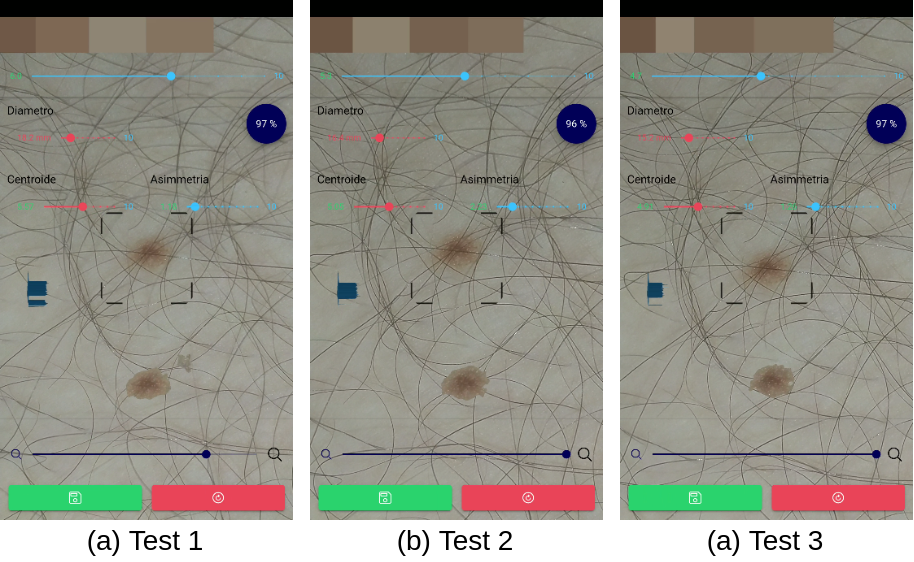
\includegraphics[scale=0.45]{figure/capitolo7/test3.png}
	\end{center}
	\caption{Analisi del nevo con peli}	
\end{figure}
\newpage
\subsection{Analisi nevo < 1cm con flash e luce artificiale} 
L'analisi di nevi di dimensione inferiore a 1 centimetro è efficace in condizioni di luce ottimale.
In Figura 7.4 l'analisi di un nevo di dimensione < di 8 millimetri.
Il tempo impiegato per l'intera analisi sulla macchina server \footnote{vedi Appendice B} è di 4.1 secondi per frame.
\begin{figure}[h]
	\begin{center}
		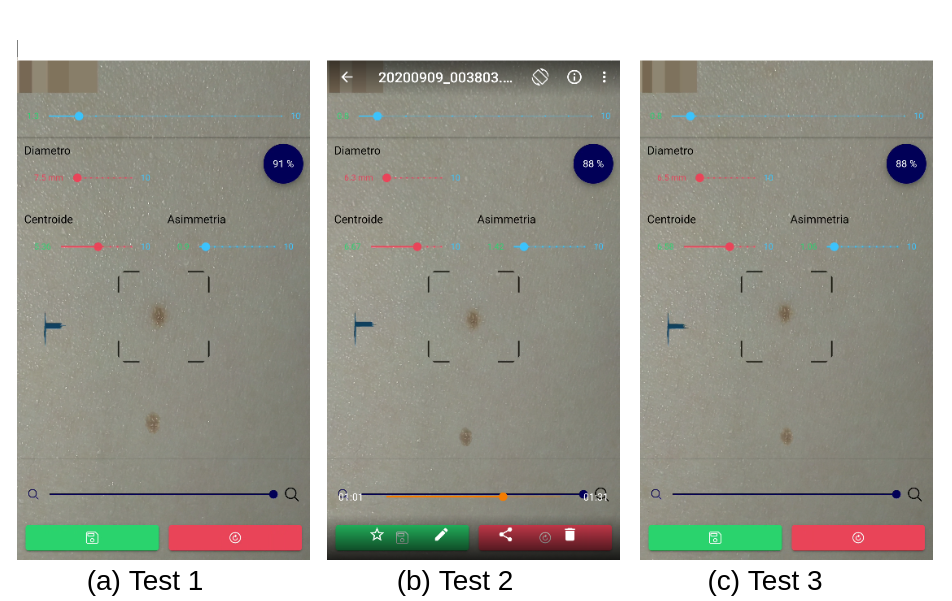
\includegraphics[scale=0.45]{figure/capitolo7/test4.png}
	\end{center}
	\caption{Analisi di un nevo nevo < 1cm}	
\end{figure}
\newpage
\subsection{Esempi di analisi errata}
Le analisi che si sono rivelate errate ed inconsistenti sono dovute ad alcuni errori di scatto da parte dell'utente ed impossibilità dell'algoritmo di segmentare correttamente il nevo.
\newline
Nella Figura 7.5 (a) la luce non era ottimale nelle direzioni opposte al nevo traendo in inganno l'algoritmo di segmentazione che non è riuscito ad individuare correttamente il nevo.
\newline
Nella Figura 7.5 (b) la posizione dello smartphone è inclinata rispetto al nevo e questo non ha permesso al classificatore di individuare il nevo correttamente.
\newline
Nella Figura 7.5 (c) la sfocatura data dallo zoom non ha permesso all'algoritmo di distinguere la pelle dal nevo.
\begin{figure}[h]
	\begin{center}
		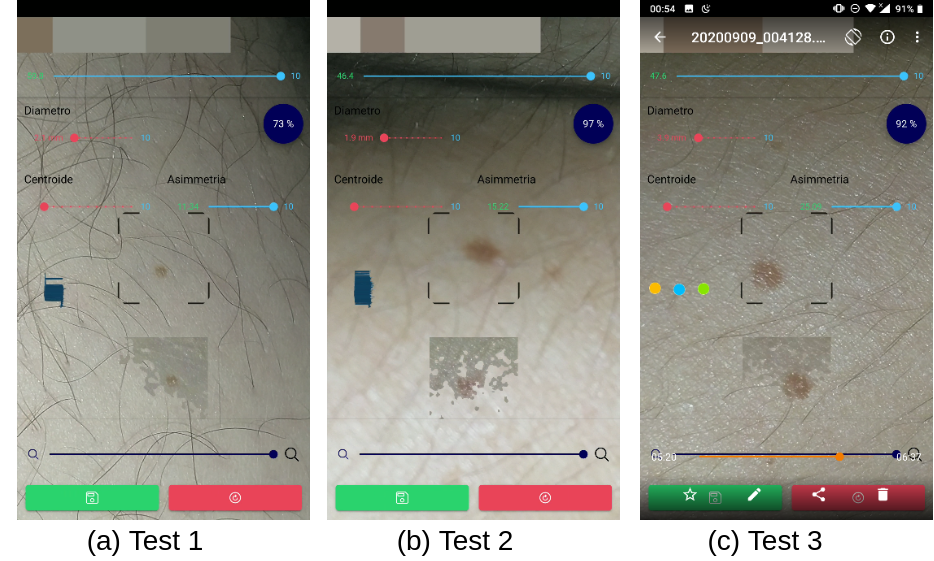
\includegraphics[scale=0.4]{figure/capitolo7/test5.png}
	\end{center}
	\caption{Esempi analisi errata }	
\end{figure}
\newpage
\subsection{Effettuare un'analisi ottimale}
Per ottenere risultati soddisfacenti ed utilizzabili in ambito clinico bisogna assicurare che i seguenti requisiti pre-analisi siano soddisfatti:
\begin{itemize}
	\item Lo smartphone deve essere posto perpendicolarmente al nevo. (Figura 7.6)
	\item La luce deve essere ottimale in ogni direzione opposta al nevo.
	\item Il nevo deve avere un colore, o un range di colori, più scuri rispetto al colore della pelle.
\end{itemize}

\begin{figure}[h]
	\begin{center}
		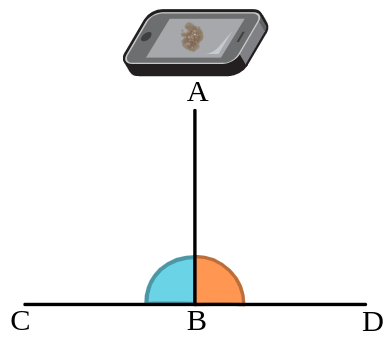
\includegraphics[scale=0.45]{figure/capitolo7/perpendicolare.png}
	\end{center}
	\caption{Smartphone posto perpendicolarmente rispetto al nevo.}	
\end{figure}
Quando una di queste tre condizioni non viene soddisfatta, i risultati possono essere non corretti e ricevere un messaggio di errore da parte dell'applicazione.
}
\chapter{Conclusioni e Sviluppi Futuri}
\label{cap:nomePrimoCapitoloTesi}
\lhead{\textbf{\rightmark}}

\indent{
	Questo capitolo presenta le conclusioni principali ed i possibili miglioramenti di questa ricerca/applicazione.
	In questo lavoro di tesi, si è sviluppato un sistema automatico per la diagnosi preliminare del melanoma basato sulla collaudata procedura medica ABCDE di uso comune.
	Il sistema proposto combina il metodo ABCD con le capacità di acquisizione ed elaborazione delle immagini degli smartphone per ottenere una diagnosi del melanoma rapida, conveniente, facilmente disponibile e altamente accurata.
	Il sistema prodotto include più moduli per la gestione delle varie fasi del metodo come: acquisizione di immagini, rimozione del rumore, segmentazione della lesione, estrazione di caratteristiche e, infine, classificazione (diagnosi).
	Nel metodo presentato, dopo aver acquisito l'immagine utilizzando la fotocamera del dispositivo questa viene inviata immediatamente al server per l'elaborazione, il quale pulisce l'immagine da eventuali peli o imperfezioni, mette in evidenza i bordi del nevo, ritaglia l'immagine, estrae le feature inerenti a asimmetria, centroide, diametro, bordi, 2D photometric stereo, fractal, dimensione frattale, colori e fa analizzare il nevo correttamente segmentato alla ConvNet.
	\begin{figure}[h]
		\begin{center}
			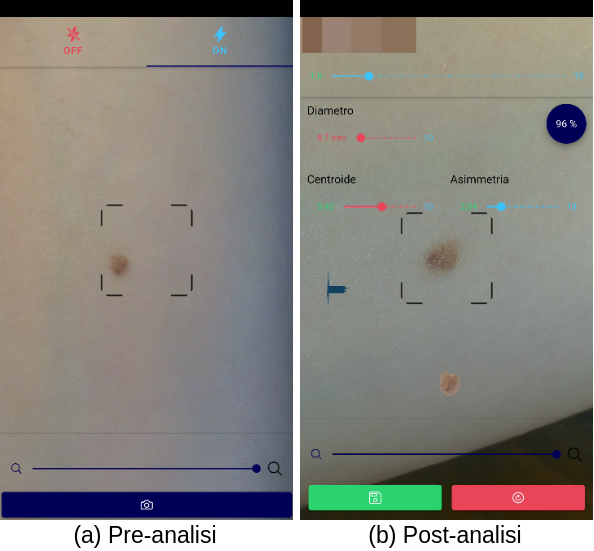
\includegraphics[scale=0.6]{figure/capitolo8/analisi.png}
		\end{center}
		\caption{Esempio dell'applicazione pre-analisi e post-analisi.}	
	\end{figure}
\newline
Gli sviluppi futuri per questo lavoro possono concentrarsi sull'aggiunta di alcune funzionalità e sul miglioramento di quelle esistenti:
\begin{itemize}
	\item Addestrare una rete neurale ad hoc per migliorare la segmentazione del nevo, che allo stato dell'arte viene effettuata con degli algoritmi che si limitano all'analisi dell'immagine ed al riconoscimento efficace dei bordi del nevo;
	\item Addestrare la rete neurale convoluzionale, che si occupa dell'analisi del melanoma, con immagini provenienti da fotocamere di smartphone;
	\item Algoritmo di riconoscimento della qualità dell'immagine sul device;
	\item Utilizzo di un sensore laser o di un riferimento sul nevo, al fine di migliorare la qualità del diametro;
	\item Sviluppare funzionalità di Evoluzione per ogni nevo e permettere al dermatologo di effettuare confronti nel tempo;
	\item Validazione dell'applicazione da parte di un dermatologo;
	\item Utilizzare le informazioni pregresse del paziente per migliorare l'analisi;
\end{itemize}
}
%Parte che richiama gli appendici

%Cambia la numerazione da numeri a lettere
\renewcommand{\thesection}{\Alph{chapter}.\arabic{section}}

\backmatter

\nocite{*}

%La bibliografia è scritta utilizzando lo stile IEEE Transaction. I contenuti bibliografici, da poi richiamare nel testo, sono descritti nel file .bib
\bibliographystyle{IEEEtran}
\bibliography{IEEEabrv,bib}

\appendix
\chapter{Appendice A - Naevus}
\label{app:nomeAppendiceA}

La scelta del nome dell'applicazione "Naevus" deriva dal latino "nævus" sostantivo della seconda declinazione maschile singolare, il cui significato è appunto "neo", "macchia naturale della pelle" oppure "voglia", in alcuni contesti può significare (in senso figurato) anche "difetto" o "macchia".
Il nome è stato preso da una celebre frase latina il cui autore è sconosciuto:
\newline
\textit{Naevus pulchram faciem non deformat},
\newline
"Un neo non guasta un bel viso".
\appendix
\chapter{Appendice B - Specifiche Tecniche}
\label{app:nomeAppendiceA}


Per i test server finali è stata scelta una macchina linux, in particolare un Lenovo Thinkpad l480 con le seguenti caratteristiche:
\begin{itemize}
	\item OS: Kubuntu 20.04 LTS (64 bit)
	\item Processore: Intel Core i5-8050U con 8 core
	\item RAM: 7,5GB
	\item SSD: Samsung 860
	\item Processore grafico: Intel UHD Graphics 620
\end{itemize}

Per i test client finali è stato utilizzato uno smartphone android, in particolare un Nokia 8 con le seguenti caratteristiche:
\begin{itemize}
\item OS: Android 9
\item Processore: Snapdragon 835
\item RAM: 4GB
\end{itemize}

Il server Django/Python è stato creato con l'ide di sviluppo PyCharm, con le seguenti librerie principali di supporto:
\begin{itemize}
\item Keras, Tensorflow
\item NumPy
\item Matplotlib
\item OpenCV
\item Scikit-learn
\item Math
\end{itemize}

Il client Ionic/Angular è stato sviluppato con l'ide di sviluppo Visual Studio Code.


\appendix
\chapter{Epilogo}
\label{app:nomeAppendiceA}
\footnotesize{
Alla fine di questi due anni esprimo queste riflessioni personali, come monito per il percorso svolto:
\begin{itemize}
\item Prima di tutto, sento il dovere di ringraziare me stesso per i risultati ottenuti, e per come li ho ottenuti
Per aver incontrato nel mio percorso persone davvero imbarazzanti ed averlo accettato. 
\item Per non aver mai mollato la data di Settembre nonostante gli ostacoli. 
\item Per tutti i sacrifici ottemperati per ottenere la massima media possibile (30L/30), senza nessun riconoscimento pecuniario da parte dell’Università (causa isee) nonostante il massimo ottenuto. 
\item Per aver fatto questo percorso con un computer di 10 anni fa, pieno di problemi, cercando di ottimizzare l’impossibile pur di far funzionare tutto. 
\item Per aver fatto la tesi con il medesimo computer che non era compatibile con gran parte delle librerie e per aver trovato, nonostante tutto, una soluzione. 
\item Per aver studiato anche di sera sul tavolo della cucina pur di non mollare.
\item Per aver servito gratis pur di ottenere trasporti come gli altri. 
\item Per non essermi tolto neanche uno sfizio e aver investito tutto nello studio.
\item Per aver cercato sempre di non gravare su nessuno, con grande rispetto per gli altri e poco per me stesso. 
\end{itemize}
Infine qualche ringraziamento:

Ringrazio Antonietta per le esose tasse pagate, per i denti e per il supporto. 

Ringrazio Gerardo per la saxo, per i denti, e per il supporto. 

Ringrazio Rita per il caffè mattutino e per il supporto (il caffè della moka che fa lei è il migliore) 

Ringrazio Carlo per il supporto e per le arrabbiature che mi causa lui e Molla, e soprattutto lo ammiro per come ha sostenuto il perido covid come il grande medico che è. (Ringrazio anche Molla)  

Ringrazio la Anna’s Family per avermi accolto sempre con le braccia aperte, Lisa in particolare per le confidenze e l’affetto mostratomi e anche la piccola Agatina. 

Ringrazio colleghi e professori che in questi due anni mi hanno aiutato a crescere e capire i miei errori. 
\newline
Un ringraziamento generale a tutte le persone che mi hanno aiutato in ogni senso in questo percorso.
\newline
\subsubsection{Dedica}
Infine vorrei dedicare, questo lavoro di tesi ad una persona che più di tutti mi ha sostenuto. 
\newline
\newline
\textbf{ANNA TOMEO}
\newline
Grazie per l’amore, l’affetto e il supporto mostratomi durante questi anni. Mi sei sempre stata vicino, sempre, quando ero in ansia prima dell’esame di Compilatori (il primo esame), quando per 3 settimane non ci siamo visti perché dovevo preparare IGES, quando dovevo preparare BD2, quando dovevo preparare SAD, o quando dovevo preparare la tesi, o quando nel periodo buio del 2020 mi hai sempre tirato su, spingendomi a dare il massimo.  
\newline
Mi sei sempre stata accanto nonostante la distanza, le litigate, i miei nervosismi strani e le mie ansie, e spero mi resterai vicino sempre. 
\newline
Grazie Anna (cici)!  }
\newline
\newline

\vspace{15mm}
\noindent
\begin{minipage}[t]{1.0\textwidth}\flushright
	%Candidato
	{\large{ \it Francesco Garofalo\\
	18/09/2018 - 12/09/2020 }}
\end{minipage}    

\end{document}